% Template for a Computer Science Tripos Part II project dissertation
\documentclass[12pt,a4paper,twoside,openright]{report}
\usepackage[pdfborder={0 0 0}]{hyperref}    % turns references into hyperlinks
\usepackage[margin=25mm]{geometry}  % adjusts page layout
\usepackage{graphicx}  % allows inclusion of PDF, PNG and JPG images
\usepackage{verbatim}
\usepackage{docmute}   % only needed to allow inclusion of proposal.tex
\usepackage{amsmath}
\usepackage{multirow}

\usepackage[nottoc,notlot,notlof]{tocbibind} % get the bibliography to be listed in the ToC as an unnumbered sectional unit

\usepackage[usenames,dvipsnames,svgnames,table]{xcolor}         % X11 colour names
\usepackage{pdfpages}
\usepackage{listings}       % Source code listings
\usepackage{courier}        % courier font
\usepackage{textcomp}       % straight quotes
\lstset{
  basicstyle=\ttfamily
, commentstyle=\color{Green}
, keywordstyle=\bfseries\color{RoyalBlue}
, showspaces=false
, showstringspaces=false
, breaklines=true
, breakatwhitespace=true
, framextopmargin=50pt
, columns=fullflexible,keepspaces
, escapeinside={(!}{!)}
, upquote=true
%, frame=bottomline
      }

\newcommand{\lml}{\lstset{language=ML,morekeywords={match,int,char,string,list,option,for,to,downto,done}}}
\newcommand{\lc}{\lstset{language=C,morekeywords={}}}
\newcommand{\lnone}{\lstset{language={},morekeywords={}}}

\raggedbottom                           % try to avoid widows and orphans
\sloppy
\clubpenalty1000%
\widowpenalty1000%

\renewcommand{\baselinestretch}{1.1}    % adjust line spacing to make
                                        % more readable

\begin{document}

\bibliographystyle{plain}


%%%%%%%%%%%%%%%%%%%%%%%%%%%%%%%%%%%%%%%%%%%%%%%%%%%%%%%%%%%%%%%%%%%%%%%%
% Title


\pagestyle{empty}

\rightline{\LARGE \textbf{Cheng Sun}}

\vspace*{60mm}
\begin{center}
\Huge
\textbf{An observable OCaml via C and \texttt{liballocs}} \\[5mm]
Computer Science Tripos -- Part II \\[5mm]
Churchill College \\[5mm]
\today  % today's date
\end{center}

%%%%%%%%%%%%%%%%%%%%%%%%%%%%%%%%%%%%%%%%%%%%%%%%%%%%%%%%%%%%%%%%%%%%%%%%%%%%%%
% Proforma, table of contents and list of figures

\pagestyle{plain}

\chapter*{Proforma}

{\large
\begin{tabular}{ll}
Name:               & \bf Cheng Sun                       \\
College:            & \bf Churchill College                     \\
Project Title:      & \bf An observable OCaml via C and \texttt{liballocs} \\
Examination:        & \bf Computer Science Tripos -- Part II, July 2017  \\
Word Count:         & \bf 11643\footnotemark[1] \\
Project Originator: & Stephen Kell                    \\
Supervisor:         & Stephen Kell                    \\
\end{tabular}
}
\footnotetext[1]{This word count was computed
by \lnone\lstinline!detex diss.tex | tr -cd '0-9A-Za-z \\n' | wc -w!
}
\stepcounter{footnote}


\section*{Original Aims of the Project}

To create an OCaml backend that can compile a useful subset of the OCaml
language to C, including for instance tuples, records, polymorphic and first
class functions. Furthermore a subset of the OCaml standard library should be
provided, and a C runtime library implemented, providing support for closures --
a feature non-native to C. The produced C code is to be integrated with
liballocs, a library tracking allocations at runtime, and should be debuggable
using liballocs to allow polymorphism to be ``seen through''.


\section*{Work Completed}

Despite the difficulty of implementing an entirely new backend into any compiler,
I have successfully created a working compiler backend translating OCaml's
\lstinline!Lambda! intermediate representation into standard C, which is capable
of compiling the \lstinline!Pervasives! and \lstinline!List! stdlib modules from
upstream as-is. Furthermore I implemented a C runtime library which provides
support for I/O, exceptions and closures, amongst others. Observability has
been demonstrated with \lstinline!liballocs!, and an extensive test and
benchmark suite demonstrates competitive performance compared to the upstream
compiler.

\section*{Special Difficulties}

None.

\newpage
\section*{Declaration}

I, Cheng Sun of Churchill College, being a candidate for Part II of the Computer
Science Tripos, hereby declare
that this dissertation and the work described in it are my own work,
unaided except as may be specified below, and that the dissertation
does not contain material that has already been used to any substantial
extent for a comparable purpose.

\bigskip
\leftline{Signed}

\medskip
\leftline{Date}

\tableofcontents

\newpage

\pagestyle{headings}

\chapter{Introduction}

OCaml is one of the most commonly used members of the ML family of functional
languages. It is popular for its expressivity, type system and performance.
My project augments the OCaml compiler with a new backend which is capable of
targetting the C programming language. The code produced by my compiler can
then be compiled with a C compiler such as gcc, and the resulting binary behaves
equivalently to the original OCaml code.

In particular, my compiler backend takes as input OCaml's \lstinline!Lambda!
Intermediate Representation. The choice of this IR over any of OCaml's other IRs
is discussed later in section \ref{why-lambda}.

\section{Motivation}

There are several motivating factors behind this project.

\begin{enumerate}
    \item \textbf{Feasibility}: I was curious whether it was technically
        possible to compile from OCaml code to C, and if so, how hard it would
        be to do so. I was also excited by the challenge of working on the
        internals of an industrial-strength compiler for the first time.
    \item \textbf{Universality of \lstinline!Lambda!}. The
        \lstinline!Lambda! IR is a fairly flexible and
        expressive target, which is rapidly garnering attention as a
        suitable target IR for compiler frontends of other languages
        \cite{dolan16}. My project attempts to implement the other direction as
        well -- that \lstinline!Lambda! is suitable for being easily translated
        into other representations;
    \item \textbf{Performance}: C has very mature toolchains that have been
        refined and optimised over tens of years. It would be nice to leverage
        the optimisations that the GCC and Clang compilers can provide for
        free;
    \item \textbf{Observability}: gdb is a very mature debugger for C, which
        far surpasses OCaml's in power. Along with enhancements brought about
        by \lstinline!liballocs!, it is now possible to observe polymorphic
        values propagating through an OCaml program. A more detailed example
        is given below;
    \item \textbf{Portability}: C can be compiled on a diverse range of
        platforms. It would be nice to know that, by using C as an intermediate
        step, OCaml code could theoretically run on these platforms with
        minimal to no changes.
\end{enumerate}

There is not as of yet a good story for debugging OCaml programs, and
observing their behaviour at runtime. The following is an example which I brought up
in my project proposal:
\lml\begin{lstlisting}
let my_rev lst =
  match lst with
  | [] -> []
  | x::xs -> List.append xs [x]

let result = my_rev [1; 2; 3]
\end{lstlisting}\lnone{}

ocamldebug, the OCaml bytecode debugger, cannot see through
polymorphism. This means that if a breakpoint is set in \lstinline!my_rev!,
ocamldebug would not be able to print out the value of the polymorphic argument
\lstinline!lst!, because its actual type is not known.

My project solves this problem via \lstinline!liballocs! -- a library
written and maintained by my supervisor, Stephen Kell.\cite{kell} This library
keeps track of runtime allocation information with low overhead. The library is
further described in section \ref{liballocs}.

There exists related prior work \cite{tarditi90} that shows that the
concept of translating from a functional language from the ML family is
feasible. However, my design and implementation will be different.  For
instance, the presented compiler generates code that uses continuation-passing
style, which I would like to avoid doing, as it harms observability --
backtraces would no longer be directly meaningful.


\chapter{Preparation}

Before starting the project, I was fairly comfortable with both the OCaml and
C languages. However, I had no experience with the OCaml compiler codebase, nor
indeed any experience in working on a project as large as it.

The vast majority of my code will be written to be built as part of the OCaml
compiler. The compiler is itself written in OCaml, and is a large and complex
code base developed over the course of over 20 years, consisting of 197k lines
of OCaml and 42k lines of C.\footnote{As counted by the \lstinline!cloc! tool.}

The OCaml compiler processes OCaml code in several phases:

\begin{center}
  \includegraphics[width=7cm]{ocamlc}
\end{center}


\section{Common types}\label{common-types}

The compiler represents the name of all variables as \lstinline!Ident.t!, which
is conceptually a tuple of the variable name string and a unique integer. Each
let binding is given its own unique \lstinline!Ident.t! -- once the frontend
has resolved variables using OCaml's scoping and shadowing rules, the rest of
the compiler has the guarantee of globally unique\footnote{Within a particular
module.} identifier names.

A \lstinline!type_expr! represents the OCaml type of a particular expression.

\section{\texttt{Parsetree} and \texttt{Typedtree}}

The very first representation used by the compiler is \lstinline!Parsetree!.
This is an Abstract Syntax Tree produced directly from the OCaml source code by
the parser. At this stage all original OCaml features are still present, before
any desugaring has happened yet. For instance, pattern matches are as
originally expressed in the source code.

The typing phase takes a \lstinline!Parsetree! and produces a
\lstinline!Typedtree!. This is the phase that ensures that all expressions are
well-typed. The \lstinline!Typedtree! is almost identical to
\lstinline!Parsetree!. The difference is that every \lstinline!expression! node
in the tree is augmented with its inferred \lstinline!type_expr!.

\section{\texttt{Lambda} IR}

For our purposes, \lstinline!Lambda! is the most important representation in
the OCaml compiler, as it is the starting point for our compiler. This
Intermediate Representation (IR) is based on a heavily augmented untyped lambda calculus.
It is a fairly low level representation, for example using integers to represent
what were originally booleans or variants.

The pass compiling \lstinline!Typedtree! into the \lstinline!Lambda! IR most
significantly desugars pattern matching into elementary conditionals and
destructuring operations. Also class and module constructs are compiled down to
operations on records.

Notably this pass does NOT:
\begin{itemize}
    \item preserve type information from \lstinline!Typedtree!. This is annoying
        for us because we would like type information for
        \lstinline!liballocs! to consume;
    \item perform closure conversion;
    \item perform uncurrying. Significantly for us this means
        partial applications and ``overapplications'' are not explicitly
    expressed as complete applications.
\end{itemize}

These issues are addressed in the implementation section.

\subsection{Why \texttt{Lambda}?}\label{why-lambda}

Quite a lot of research was done into the various intermediate representations
in the OCaml compiler before starting my project. In the end, none of the
Intermediate Representations were deemed perfect, but \lstinline!Lambda! was the
closest starting point to what I wanted.

\begin{enumerate}
  \item \lstinline!Parsetree! and \lstinline!Typedtree! are not appropriate as a starting point for my compiler. This
is because no desugaring has been performed yet, which means that there are too
many cases and constructs that would have to be handled;
  \item \lstinline!Clambda! (an IR that is part of the OCaml native compiler)
    is more suitable as a starting point, because it represents closures explicitly. However it is
    even harder to retrieve type information from than \lstinline!Lambda!. Although \lstinline!Lambda! doesn't
    preserve \lstinline!type_expr!s for every expression, some specific
    information, in the form of ``events'' (see section \ref{events}) is stored for the benefit of the ocamldebug bytecode debugger.
    These events are dropped in \lstinline!Clambda!.
\end{enumerate}

\subsection{Introduction to \texttt{Lambda}}\label{introduction-to-lambda}

Each OCaml file implicitly defines a module, whose name is the same as the
filename capitalised. For instance, \lstinline!foo.ml! defines a module named
\lstinline!Foo!.

At the toplevel, there are two different types of let statement. Let-statements
which define functions have bodies should not be executed immediately -- only
when the function is called. All other let-statements should run exactly once
when the module is loaded for the first time. For instance:
\lml\begin{lstlisting}
(* function -- not run immediately, exported *)
let foo () = [ 3 ; 2 ; 1 ]

(* ignored result -- run immediately, discarded *)
let _ = foo ()

(* variable -- run immediately, exported *)
let bar = List.sort (-) (foo ())\end{lstlisting}\lnone

This will get translated into the following (abridged) \lstinline!Lambda! code.
\lml\lstset{numbers=left}\begin{lstlisting}
Lseq (
  Lprim (Popaque, [ Lprim (Pgetglobal, [ "List" ]) ]),
  Llet (
    foo_1199,
    Lfunction ([ param_1255 ], ...),
    Lseq (
      Lapply {
        ap_func = foo_1199,
        ap_args = [ Lconst (Const_base (Const_pointer 0)) ]
      },
      Llet (
        bar_1200,
        Lapply {
          ap_func =
            Lprim (Pfield 40, [
              Lprim (Pgetglobal, [ "List" ])
            ]),
          ap_args = [ ... ]
        },
        Lprim (Pmakeblock (0, Immutable), [foo_1199, bar_1200])
      )
    )
  )
)\end{lstlisting}\lnone\lstset{numbers=none}

There are several things to note about the \lstinline!lambda! tree produced.
\begin{enumerate}
  \item \lml\lstinline!let!\lnone{} gets translated to \lstinline!Llet!, as can
    be seen on lines 3 and 11 of the output. The tree ends up very right-side heavy, as each
    \lstinline!Let! constructor takes as
		its last argument a \lstinline!lambda!
    representing the rest of the module. This mirrors the form
    of a (non-toplevel) \lml\lstinline!let ... in ...!\lnone{} expression in OCaml,
    in contrast to a more imperative style \lstinline!var ...; var ...;!.
    Although one does not write the \lml\lstinline!in!\lnone{} keyword
		for let-statements at the top-level, under the hood it desugars to this form regardless.
  \item All variable references are represented using \lstinline!Ident.t! (see
    \ref{common-types}), denoted here using an underscore between name and numeric
    identifier.
  \item On line 7, the \lstinline!foo! function is applied using
    \lstinline!Lapply!, which takes a record containing (amongst other things)
    the function and the arguments to apply.
  \item On lines 13--19, \lstinline!List.sort! is applied. Note how this requires
    accessing the globally defined \lstinline!List! module object. Also
    note that nowhere does the name ``\lstinline!sort!'' appear.

    The OCaml compiler compiles modules to records at the \lstinline!Lambda!
    level. These are stored as blocks of contiguous word-sized values, and are
    indexed into by an integer offset (using the \lstinline!Pfield! primitive). The
    order of values in the record is well defined by the OCaml compiler, so that
    other modules that link against it know the mapping from exported variable
    name to field offset.

    In this case the compiler knew that \lstinline!List.sort! was the 40th exported
    variable in the \lstinline!List! module.
  \item Line 20 constructs the ``return value'' of the \lstinline!lambda!
    expression. This is a record, representing the currently compiled module
    object, which contains the variables and functions that the module exports.

    Note that not all variables and functions are necessarily exported --
    exports can be restricted by the \texttt{.mli} file if present.
\end{enumerate}

\section{Starting point}

The project will be focused on creating a new ``backend'' for the OCaml
compiler, so I will build on the existing code of the rest of the compiler.
This includes using preexisting code for lexing, parsing and typing of OCaml programs, as
well as the transformation from the typed AST to the \lstinline!Lambda! Intermediate
Representation that we will be using.

In order to provide a standard library to compile programs against, I used
the existing OCaml \lstinline{stdlib}. However, the C runtime
library was completely written by myself.

I did not make use of either \lstinline{cil}or \lstinline{libffi} as suggested
in my project proposal. The reason behind this is explained in sections
\ref{investigating-c-ast} and \ref{investigating-closure}. All of the
functionality they would have provided was instead manually implemented by
myself.

I did make use of \lstinline!liballocs!, described below (section \ref{liballocs}).

\section{Investigating C AST representations and output}\label{investigating-c-ast}

My compiler is required to output C code, so a representation of C
is required that allows for easy manipulation. My supervisor suggested the
use of \lstinline!cil!, a C ``intermediate language'' which is capable of
semantically representing all C programs using a minimised subset of the language.

I came to the conclusion that this wouldn't be a good fit for my project, because
 CIL is, in a sense, trying to accomplish the opposite of what I want. CIL
 tries to represent a minimal subset of C, and allow transformations to be
 performed on this. On the other hand I'd like to represent the useful subset
 of C which I can use to compile OCaml constructs to.

In addition, I anticipated that I may need more fine-grained control, or custom
features, to be represented in my AST. Hence I ended up going with a hand-rolled
representation.


\section{Investigating closure support in C}\label{investigating-closure}

Supporting closures in C was one of the earliest identified points of difficulty.
Early on my supervisor recommended that I look at the approach introduced by
Breuel \cite{breuel88}. After reading and understanding the paper I had a
better understanding of the problem and was fairly confident I could implement
the proposed solution.

Even so, some preliminary investigation was done towards possible external
libraries that could be used to provide this support for me. One of these,
\lstinline!libffi!, was also suggested by my supervisor.

I came to the conclusion that \lstinline!libffi!'s API was too generic
and complex for the very specific use case that I had in mind. In addition, I
wasn't sure whether the library would give me enough control. Finally, I wanted
to take on the challenge of implementing closures myself, so that I could gain
a better understanding of the technique.

\section{\texttt{liballocs}}\label{liballocs}

I will use the open-source \lstinline{liballocs}, written by Stephen Kell.
\lstinline!liballocs! is a C library (and accompanying toolchain wrapper)
written and maintained by my supervisor, Stephen Kell. The library transparently
keeps track of the sizes and types of all allocated memory, with no
modifications required. Given an arbitrary valid pointer, \lstinline!liballocs!
can return information about the start and the extend of the corresponding
allocated block, and also the C type of the allocation.

As the library and toolchain were designed to be drop-in replacements for gcc or
clang, I didn't spend very much preliminary time studying the library.



\chapter{Implementation}

The stages of my C compiler backend are as follows:

\begin{center}
  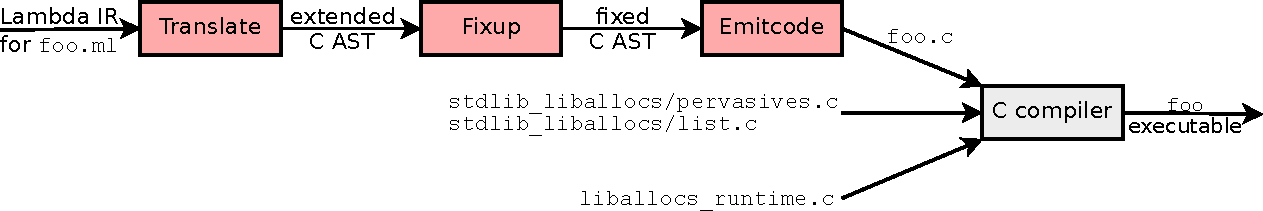
\includegraphics[width=16cm]{compiler_structure}
\end{center}

\section{\texttt{module C}: the extended C abstract syntax tree datatype}\label{module-c}

I have defined a datatype representing a C-like syntax tree. Not all C features
are modelled -- only the constructs that my compiler needs to produce.

The tree datatype is more expressive than standard ANSI C. These extra
features are rewritten into standard C in a later pass, as detailed later in
section \ref{module-fixup}.

The following datatypes are defined for use inside my compiler. Their output representations in the C code are described in later sections.

\begin{itemize}
  \item
    \lstinline!C.ctype! represents a C type. Notable constructors include:

    \begin{itemize}
        \item \lstinline!C_Int!;
        \item \lstinline!C_Double!;
        \item \lstinline!C_Pointer of C.ctype!;
        \item \lstinline!C_Value!, a word-sized type capable of representing
          any OCaml value -- described later in section \ref{value-representation};
        \item \lstinline!C_Struct of Ident.t * (C.ctype * string) list!;
        \item \lstinline!C_FunPointer of C.ctype * C.ctype list! taking return
            type and argument types.
    \end{itemize}

    For instance, the type of a function pointer \lstinline!void (*)(double *)! is
    represented in my OCaml code as
    \lstinline!C_FunPointer (C_Void, C_Pointer C_Double)!.
  \item
    \lstinline!C.expression! represents an expression -- program fragments that
    evaluate to a value (possibly of type \lstinline!void!). Notable
    constructors for this datatype include:
    \lml\begin{itemize}
        \item Data literals of various types:
            \begin{itemize}
                \item \lstinline!C_IntLiteral of Int64.t!
                \item \lstinline!C_StringLiteral of string!
                \item \lstinline!C_FloatLiteral of string!\footnote{Floats are
                    always represented in the OCaml compiler as strings, to
                    prevent rounding errors.}
                \item \lstinline!C_CharLiteral of char!
                \item \lstinline!C_PointerLiteral of int!\footnote{This
                    doesn't take \lstinline!int64! as might be expected, as it
                    is used to represent lambda's \lstinline!Const_pointer of int!,
                    which seems only to be used by the compiler to represent
                    \lstinline!NULL!.}
            \end{itemize}
        \item Variables. Two different kinds are distinguished:
          \begin{itemize}
            \item \lstinline!C_Variable of Ident.t! takes an identifier (see section
              \ref{common-types}), and is used for all local variables
              originating from OCaml code. The variables are formatted suffixed
              with their unique integer: \lstinline!variablename_1234!.
            \item \lstinline!C_GlobalVariable of string! takes a string and
              outputs it verbatim -- there is no integer suffix. The compiler
              generates these references when it needs to reference internal
              functions, such as \lstinline!ocaml_liballocs_close! (see section
              \ref{closures-runtime-support}). Cross-references to other
              modules also use these.
          \end{itemize}
        \item \lstinline!C_FunCall of C.expression * C.expression list!
            represents function calls as an expression evaluating to the
            function to be called, and the list of arguments. See section \ref{functions}.
        \item \lstinline!C_BinaryOp of string * expression * expression!
            represents all arithmetic and logical binary operations.
    \end{itemize}\lnone

    For instance, the expression \lstinline!foo + 2! is represented as
    \lml\begin{lstlisting}
C_BinaryOp (C_Variable foo, "+",
            C_IntLiteral (Int64.of_int 2))\end{lstlisting}%
    (where \lstinline!foo : Ident.t! is the identifier representing the name of the
    \lstinline!foo! variable).

    \lnone
  \item
    \lstinline!C.statement! represents a statement -- language constructs such as:
        \lml\begin{itemize}
            \item \lstinline!C_If of expression * statement list * statement list!
            \item \lstinline!C_While of expression * statement list!
            \item \lstinline!C_Return of expression option!
            \item etc.
        \end{itemize}\lnone
        Note that statements typically contain one or more expressions, whereas
        expressions in standard C cannot contain statements.

  \item
    \lstinline!C.toplevel! represents a function or global variable declaration/definition at the toplevel.
\end{itemize}

\subsection{Inline statements}\label{c-inline-statements}

The fact that C language makes a distinction between ``statements'' and
``expressions'' makes it less expressive than OCaml, as all core language
features in OCaml can be used as expressions. For instance, consider the
translation of the following OCaml code:

\lml\begin{lstlisting}
let x = if foo then (if bar then 1 else 2) else 3\end{lstlisting}\lnone{}

Clearly a direct translation of this wouldn't be possible, as \lstinline!if!
statements cannot be used as expressions in C. The ternary operator
\lstinline!?:! exists in C as an expression analogue of \lstinline!if!.
However, it isn't used by my compiler for two reasons.  Firstly in the
interests of readability -- nested ternary operators get hard to read very
quickly. The second reason is that debuggability of if statements would be
hampered by the fact that debuggers tend not to be able to single-step easily
from the condition to the body.

Even if the ternary operator were used, there are other statements that
cannot be made into expressions as easily. An example is the let-statement,
which translates to variable declarations in C. Hence, a solution to this
general problem would still be required.

The way that we handle this is by extending our \lstinline!C.expression! so
that statements can used as ``pseudo-expressions''.  We add a new constructor
\lstinline!C_InlineRevStatements of C.statement! to the
\lstinline!C.expression! type, which allows us to use any block of C statements as if it
were an expression.

By doing this, our example from above can be translated directly, simply by
wrapping the \lstinline!C_If! statement up as an ``inline statement''. The
inline statement evaluates to the ``value'' of the last statement in the block.

We fix up the presence of these in a later phase -- see section \ref{module-fixup}.

\section{Runtime value representation}\label{value-representation}

In the produced C code, \lstinline!ocaml_value_t! is a type which is capable of
representing any OCaml value. This type corresponds to the \lstinline!C_Value!
datatype in my compiler. This type is required to represent polymorphic OCaml
types: for instance a function with a parameter of OCaml type \lml\lstinline!'a!\lnone{}
would take a C parameter of type \lstinline!ocaml_value_t!.\footnote{As it
turns out, it's easier to represent \textit{all} OCaml values as values of this
type, not just polymorphic ones.}

A simple way of implementing this type is to make all OCaml values boxed. This means
that everything is allocated on the heap, and the variables of type
\lstinline!ocaml_value_t! are all just pointers into the heap. However this has
several significant downsides.

One downside of using boxed objects is that the extra indirection required to
access each variable is very slow. Another is that boxing small types, such as
integers, requires twice as much memory -- one word-sized integer on the heap
and the word-sized pointer to it.

Because of this, I decided to make my \lstinline!ocaml_value_t! representation
capable of storing some types of value unboxed. However, we would still like
\lstinline!ocaml_value_t! to be exactly 64-bits in size, so that it fits into a
register. A technique is needed to squeeze both pointers and \textit{immediates}
(unboxed values such as integers and floating point numbers) into just 64 bits.
Various such techniques have been used over the years by high-performance
compilers and interpreters:
\begin{enumerate}
  \item \textbf{untagged values}, as used by the D programming language, for
    example. This ``technique'' simply represents each type of value as itself.
    Note that there is no way to tell what type the value is just from inspecting the value itself.

    Although OCaml is an example of a statically typechecked language which would
    still be correct without runtime type information\footnote{Almost -- OCaml's
    ``polymorphic comparisons'' feature require a limited form of value tagging
    to support structural comparison.}, this approach is not used by the upstream
    compiler. This is because any garbage collector that works with such a
    value representation must be conservative, which has many
    disadvantages.
  \item \textbf{tagged pointers}, as used by OCaml's upstream compiler, the V8
    JavaScript engine, and many others. This technique steals the least
    significant bit of each 64-bit value to use as a ``tag bit'', signifying whether
    that value is boxed or not. In OCaml's scheme, an unset tag bit indicates
    that the value is a pointer, and a set bit indicates an immediate 63-bit integer.
    The reason this works is because pointers to valid OCaml objects are always
    8-byte aligned, which means that all valid pointers have the bottom
    three bits zeroed. The disadvantage of this representation is that there is
    no space to represent doubles -- they must be boxed.
  \item \textbf{NaN boxing}, as used by WebKit's JavaScriptCore engine,
    SpiderMonkey and LuaJIT. This is the scheme I chose to use, because unlike
    the tagged pointers approach, both immediate integers and doubles can be
    represented. The details are described in the next section.
\end{enumerate}

\subsection{NaN boxing}\label{nan-boxing}

NaN boxing is a surprising technique which, in contrast to the other
techniques described previously, has the following desirable properties:
\begin{enumerate}
    \item has the ability to store IEEE 754 floating point numbers (\lstinline!double!s) unboxed;
    \item provides additional space to store user-space pointers\footnote{On 64-bit
      Linux, user-space pointers are only 48-bits long. The top bits are always
      zero, to distinguish them from kernel pointers, which have top bits set to
      one.};
    \item provides even more additional space (which we use to store 50-bit integers);
    \item none of these three ranges overlap: a simple comparison test can be
      used to distinguish which of the three types a given NaN boxed value is.
\end{enumerate}

NaN boxing allows us to represent doubles unboxed. Our implementation of NaN
boxing was inspired by JavaScriptCore's \cite{jscore}, however the exact choice
of encoding and implementation details are original.

The representation of IEEE 754 double-precision floats is shown in figure \ref{fig-ieee754}.
\begin{figure}[h]
  \centering
  \includegraphics[width=14cm]{ieee754}
  \caption{The memory format of an IEEE 754 double floating point value.}
  \label{fig-ieee754}
\end{figure}

Not-a-Number (NaN) values in IEEE 754 double values take
up a needlessly large range of the 64-bit space. In
particular, any of the $2^{53}-1$ numbers with an exponent of \texttt{0x7FF} and
non-zero mantissa is a NaN value. However, there are actually only four
different NaNs: plus or minus quiet ($\pm$qNaN) and signalling ($\pm$sNaN).
Modern CPUs only ever use one specific (canonical) bit representation for each
type of NaN, which leaves the rest of the range to embed other types of values
into (see the first two columns of table \ref{table-nan-range}).

Before we store the embedded value into the \lstinline!ocaml_value_t!, we perform
one final adjustment: add $2^{48}$ to the integer representation of the double. This
gives us the ``in-memory representation'' shown in the third column of table
\ref{table-nan-range}. The purpose of this is so that the final representation
of pointers is exactly the same as their raw representation (with top 16 bits clear).
This means the common operation of dereferencing a pointer \lstinline!ocaml_value_t!
requires no additional overhead.

\begin{table}
  \centering
\begin{tabular}{c | c | c}
  \textbf{purpose} & \textbf{double space representation} & \textbf{in-memory representation} \\ \hline\hline
    \rowcolor[rgb]{0.7,0.7,0.7}$-{}$infinity & \lstinline!fff0! \lstinline!000000000000! & \lstinline!fff1! \lstinline!000000000000! \\ \hline
    unused  & \vdots & \vdots \\
    \rowcolor[rgb]{0.7,0.7,0.7}$-{}$sNaN (canonical)  & \lstinline!fff4! \lstinline!000000000000! & \lstinline!fff5! \lstinline!000000000000! \\
    unused  & \vdots & \vdots \\ \hline
    \rowcolor[rgb]{0.7,0.7,0.7}$-{}$qNaN (canonical)  & \lstinline!fff8! \lstinline!000000000000! & \lstinline!fff9! \lstinline!000000000000! \\
    unused  & \vdots & \vdots \\ \hline
    \rowcolor[rgb]{0.7,1.0,0.7} & \lstinline!fffb! \lstinline!000000000000! & \lstinline!fffc! \lstinline!000000000000! \\
    \rowcolor[rgb]{0.7,1.0,0.7} & \vdots & \vdots \\
    \rowcolor[rgb]{0.7,1.0,0.7}\multirow{-3}{*}{Integers (50-bit space)} & \lstinline!fffe! \lstinline!ffffffffffff! & \lstinline!ffff! \lstinline!ffffffffffff! \\ \hline
    \rowcolor[rgb]{0.7,1.0,0.7} & \lstinline!ffff! \lstinline!000000000000! & \lstinline!0000! \lstinline!000000000000! \\
    \rowcolor[rgb]{0.7,1.0,0.7} & \vdots & \vdots \\
    \rowcolor[rgb]{0.7,1.0,0.7}\multirow{-3}{*}{Pointers (48-bit space)} & \lstinline!ffff! \lstinline!ffffffffffff! & \lstinline!0000! \lstinline!ffffffffffff! \\
\end{tabular}
\caption{Table showing negative NaN space. There is a similar unused space
inside the positive NaN region, but we don't use that. Values which we cannot
reuse are coloured grey, and ranges which we've reserved for ourselves are
coloured green.}\label{table-nan-range}
\end{table}

Notice that for efficiency, the ``in-memory representation'' of integers was
chosen such that the original integer can be recovered exactly using a single
bit-mask operation.

The actual C type definition of \lstinline!ocaml_value_t! is the following union:
\lc\begin{lstlisting}
union _ocaml_value_t;

typedef union _ocaml_value_t *generic_datap_t;
typedef union _ocaml_value_t (*generic_funcp_t)();

typedef union _ocaml_value_t {
    intptr_t        i;
    generic_datap_t p;
    generic_funcp_t fp;
} ocaml_value_t;
\end{lstlisting}\lnone
Note that we use the \lstinline!i! field for both integers and doubles. This is
because doubles need to be reinterpreted as integers in order to apply the
$2^{48}$ shift as described previously.

Also note that data pointers and function pointers are accessed using different
union fields, despite the fact that both are 64-bit pointers into the same
address space on Linux. This is a quirk of C: casting between these two types
of pointers is undefined behaviour. Interestingly \lstinline!gcc! will indeed
miscompile code that casts betwen these two types.

We define some helper macros in C:
\begin{enumerate}
    \item \lstinline!NEW_I!, \lstinline!NEW_D!, and \lstinline!NEW_P! allow us to
    wrap raw integer, double or pointer values into new \lstinline!ocaml_value_t!.
    These perform the encoding step as described previously. For instance,
    \lstinline!NEW_D! is defined by viewing the double as an integer, and
    adding $2^{48}$, as follows:

\lc\begin{lstlisting}
static intptr_t __double_encode(double x) {
    union {
        double d;
        intptr_t i;
    } s = {.d = x};
    return s.i + (1LL<<48);
}
#define NEW_D(v) ((ocaml_value_t){.i = __double_encode(v)})\end{lstlisting}\lnone

    \item \lstinline!GET_I!, \lstinline!GET_D!, and \lstinline!GET_P! allow us to
        unwrap an \lstinline{ocaml_value_t} back into a raw integer, double or
        pointer value respectively. For instance, \lstinline!GET_D! is defined
        as:
\lc\begin{lstlisting}
#define GET_D(v) (__double_decode((v).i))\end{lstlisting}\lnone
        where \lstinline!__double_decode! is the inverse of the \lstinline!__double_encode! operation defined previously.

    \item \lstinline!IS_I!, \lstinline!IS_D!, and \lstinline!IS_P! allow us to
        discriminate which type of value is wrapped inside an
				\lstinline{ocaml_value_t}. This is done by simple integer range tests
				-- for instance:
\lc\begin{lstlisting}
#define IS_I(v) \
  ((uintptr_t) (v).i >= 0xfffc000000000000ULL)\end{lstlisting}\lnone
\end{enumerate}

\subsection{50-bit integer arithmetic}\label{50-bit-integer}

NaN boxing limits our integers to be 50-bit sized. Luckily, the size of OCaml's
standard unboxed integer is deliberately left unspecified -- in fact the
upstream compiler uses either 31-bit or 63-bit integers depending on the
platform.

Interestingly, most native word-sized arithmetic operations work correctly on
non-word-sized integers, due to the properties of modular arithmetic and twos
complement representation. For instance, consider two 50-bit integers stored in
64-bit registers, with arbitrary values for the top 14 bits. A 64-bit multiply
of the two registers will generate the correct answer in the bottom 50 bits of
the resulting register.

The only cases where non-word sized integers need careful treatment are
operations where more significant bits in the input can influence less
significant bits in the output, such as the right shift and divide operations.
OCaml has two shifts:
\begin{itemize}
  \item logical shift, where the shifted-in bits are set to zero;
  \item arithmetic shift, where the shifted-in bits are set to the sign bit.
\end{itemize}

Logical right shift (lsr) is relatively simple -- first set the top 14 bits to
zero by using a mask, then perform a native-width logical right shift.

Arithmetic right shift (asr) and division are trickier. We first need to
``clean up'' the top 14 bits by extending our real sign bit (bit 49) into them.
This can be achieved using the following C bitfield trick:
\lc\begin{lstlisting}
static intptr_t __sext50(intptr_t x) {
    struct {
        intptr_t x : 50;
    } s = {x};
    return s.x;
}
\end{lstlisting}\lnone

This defines a bitfield integer which is logically 50 bits long. We write
\lstinline!x! into it, and then read out a value of type \lstinline!intptr_t!
(which is 64 bits long). C semantics cause the 50-bit field to be sign extended
into the rest of the integer, which is exactly the operation we want.\footnote{
The compiler will likely implement this under the hood as
\lstinline!(x lsl 14) asr 14!.}

\subsection{Casting \texttt{ctype}s}

In order to work smoothly with both wrapped and unwrapped expressions in my compiler,
I define a NaN-box-aware cast operation that transforms between the two when required.

First, define the \textit{kind} of a non-\lstinline!C_Value! \lstinline!ctype!
as one of the following: integer-like, float-like, data-pointer-like, or
function-pointer-like. The operation of casting from an expression of \lstinline!ctype! ``source''
into type ``target'' is defined as below:

\begin{enumerate}
  \item If source and target are the same, nothing needs to be done;
  \item If source is \lstinline!C_Value! and target is not, then we need to
    unwrap the expression. Assuming the cast is valid, then use the appropriate
    \lstinline!GET_*! macro to retrieve the original value;
  \item If target is \lstinline!C_Value! and source is not, then we need to
    wrap the expression using the appropriate \lstinline!NEW_*! macro;
  \item Otherwise use a C cast to the target type.
\end{enumerate}

\section{\texttt{module Translate}: compilation from lambda IR to C AST}

The implementation of \lstinline!Translate! is done via a recursive tree-walk
over the \lstinline!Lambda! tree. Two mutually recursive functions each
target the different types of C program fragment:

\lml\begin{lstlisting}
val lambda_to_texpression :
  Lambda.lambda -> C.ctype * C.expression
val lambda_to_trev_statements :
  Lambda.lambda -> C.ctype * C.statement list\end{lstlisting}\lnone{}

Note that each translation function also returns the \lstinline!C.ctype! of the expression or statement. This is for the purposes
of casting, as defined earlier. For instance, if an OCaml expression
evaluates to an \lstinline!ocaml_value_t!, and is subsequently used in an if
condition, the value must first be unwrapped into a boolean.

Because of the flexibility of the \lstinline!cast! mechanism, and the
expressivity that \lstinline!C_InlineRevStatements! provides, the actual
recursive translation from \lstinline!Lambda! is actually fairly straight-forward.

To illustrate, the following is the implementation of
\lstinline!lambda_to_trev_statements! for OCaml if statements:
\begin{lstlisting}
...
| Lifthenelse (l,lt,lf) ->
  let cexpr_cond = cast C_Bool (lambda_to_texpression l) in
  let trev_t = lambda_to_trev_statements lt in
  let trev_f = lambda_to_trev_statements lf in
  let (ctype, sl_t, sl_f) = unify_revsts ~hint:"ifthenelse" trev_t trev_f in
  ctype, [C_If (cexpr_cond, sl_t, sl_f)]
...\end{lstlisting}

(The use of \lstinline!unify_revsts! picks the more general type out of the
types of the true and false statement blocks, and casts the other so that it
evaluates to the general type.  The overall return type of the if statement is the
more general one.)

Unfortunately the lambda IR is not documented anywhere, so the semantics
of these instructions were divined through reverse engineering and code diving.

\subsubsection{Primitive operations}

``Primitive'' operations in \lstinline!Lambda! are represented by
\begin{lstlisting}
Lprim (primitive, args)\end{lstlisting}
where \lstinline!args! are a list of \lstinline!lambda! terms, and
\lstinline!primitive! is a type of operation. Most primitive operations map
fairly simply to C constructs. In total I handle 49 different primitives.
Notable \lstinline!primitive!s include:
\begin{enumerate}
  \item unary and binary operations on integers and doubles;
  \item \lstinline!Praise! throws an exception (see section \ref{exceptions});
  \item \lstinline!Pstringlength! evaluates to the length of a C-style string. I translate this to a call to \lstinline!strlen!;
  \item \lstinline!Pmakeblock! performs an (untyped) allocation of a given size.

    This is more complex than the others, as this primitive specifies
    the values that the newly allocated memory is initialised to. Hence we need
    to recursively translate these values, as well as wrapping up the
    statements required for allocation and initialisation into a single
    ``expression''.
    
    Things are made even more complex in the case that this
    \lstinline!Pmakeblock! refers to a mutually recursive let-binding. We have
    to split up the allocation and initialisation phases: see section \ref{mutually-recursive-values}.
\end{enumerate}


\subsubsection{Events}\label{events}

Events are a special \lstinline!Lambda! constructor which contains type
information on the let bindings in scope at the point of the event. These are
used by the OCaml debugger.

It's not possible to make use of events during the translation step itself,
as an event describing a particular binding can be encountered too late during
the recursive traversal. For instance the event describing the types of arguments
to a function can be buried inside the body of the function, whereas
translation needs to know the type at the point the arguments are first encountered.

We perform a step before compilation proper, which I called ``event scraping''.
This is a complete traversal of the \lstinline!Lambda! tree, where all non-event
nodes are ignored. Type expressions in all events encountered are cached in a
``variable library,'' a hash table mapping variable identifiers
(\lstinline!Ident.t!) to their types. Once event scraping is complete, we have
information about the types of all variables defined in the entire module.

\subsubsection{Inline function definitions (lambdas)}\label{c-inline-functions}


OCaml allows one to define new functions anywhere, for example in the following example:
\lml\begin{lstlisting}
let x = (fun x -> x + 1) 41\end{lstlisting}\lnone{}
However, C does not -- all
functions must be defined at the toplevel. The way that we handle this is similar
to how we expressionify statements: by introducing an ``inline function
definition'' pseudo-expression. After fixup the function body will get pulled
out to the toplevel, and the pseudo-expression replaced with the name of the
newly created function.

Note that this does not work if the function is not closed (i.e. depends on values
from its environment). In this case we must create a closure at runtime instead, and
this is the subject of section \ref{closures}.

\section{\texttt{module Fixup}: translation from extended-C AST to valid C AST}\label{module-fixup}

The purpose of fixup is to eliminate inline statements and inline function
definitions. Similar to \lstinline!Translate!, the implementation is done via a
recursive tree-walk. Mutually recursive functions each visit
different types of nodes:

\begin{lstlisting}
var fixup_expression :
  Fixup.t -> C.statement list -> C.expression ->
  C.statement list * C.expression
var fixup_rev_statements :
  Fixup.t -> C.statement list -> C.statement list ->
  C.statement list
\end{lstlisting}

Each fixup function takes an accumulator of type \lstinline!C.statement list!,
which is a (reversed) list of statements to be placed before the expression or
statement currently being fixed.

As we traverse the AST, fixed statements get pushed onto the front of the accumulator.
When we encounter a \lstinline!C_InlineRevStatements!, we first push the
inlined statements onto the accumulator, and replace the expression with the
expression that the inlined statements evaluate to. Then, once there are no more
statements to fix, we reverse the accumulator and return the result.

To illustrate, consider fixing the following (where square brackets indicate inlined statements):
\lc\begin{lstlisting}
x = [
  if (a) { 42; } else { foo(); }
];\end{lstlisting}\lnone{}
This turns into the following after fixup:
\lc\begin{lstlisting}
int __deinlined;
if (a) { __deinlined = 42; } else { __deinlined = foo(); }
x = __deinlined;\end{lstlisting}\lnone{}

Care must be taken to pass a new empty accumulator when entering a new scope,
for example when fixing the bodies of if, for and while loops. Also, care must
be taken to preserve evaluation order -- statements must be consed onto the
head of the accumulator in the order that they must be evaluated.

Inline function definitions are easier to handle. All such functions are pulled
out and placed at the top of the C file in the order they were encountered.
Each ``inline function definition'' pseudo-expression is replaced with the
identifier of the newly-created function.

\section{\texttt{module Emitcode}: outputting C AST to a file}\label{emitcode}

\lstinline!Emitcode! is responsible for stringifying the AST into valid C code,
and outputting this to the target file. The majority of code is straightforward
string manipulation, using recursion to traverse the tree. There are two things
to note:
\begin{enumerate}
  \item Not all OCaml identifiers are legal in C -- for instance, the apostrophe character
    is allowed by OCaml. C only allows alphanumeric characters and underscore.
    We encode illegal identifiers as follows:
    \begin{enumerate}
			\item If an identifier contains at least one illegal character, suffix
				the identifier with an underscore. Because identifiers normally always end with
				their unique number, encoded identifiers will never collide with a legal
				identifier;
			\item For each illegal character, expand it to the character sequence
				\lstinline!"_uXXXX_"! where \lstinline!XXXX! is the hexadecimal character code
				of the illegal character.
    \end{enumerate}
	\item Certain variable declarations require special casing to format properly. In particular,
    a function pointer \lstinline!x! with type \lc\lstinline!void (*)()!\lnone{} is not defined as:
    \lc\begin{lstlisting}
    void (*)() x;\end{lstlisting}\lnone{} as might be expected, but instead as
    \lc\begin{lstlisting}
    void (*x)();\end{lstlisting}\lnone{}
\end{enumerate}

\section{Basic constructs}

\subsection{Functions and complete application}\label{functions}

OCaml functions map directly to C functions, with complete function application
corresponding to function calls. Currently all functions have arguments and
return values of wrapped type \lstinline!ocaml_value_t!. This is to facilitate
calling functions in another module -- at the \lstinline!Lambda! level I do
not have type information about functions in other modules.

Mutually recursive functions are simply handled in C. All that is required is
that the functions in question are predeclared before they are defined.

Partial application and closures are discussed later in section \ref{closures}.

\subsection{Mutually recursive definitions}\label{mutually-recursive-values}

Consider the OCaml expression

\begin{lstlisting}
let rec a = 1::b and b = 2::a in ...
\end{lstlisting}

This defines a mutually recursive \textit{value} -- creating a infinite
(cyclic) list of period 2. The value of \lstinline!a! will be
\lstinline!1::2::1::2::1:: ...!

In order to ensure correct semantics even in the presence of mutually recursive
value definitions, my compiler separates the variable definition process into
three phases:

\begin{enumerate}
  \item \textbf{Allocation}: first the required memory for each variable are
    allocated using \lstinline!malloc!;
  \item \textbf{Closure creation} (if necessary): at this point the memory
    addresses of variables are known, and so can be frozen into closures as
    needed. The process is described in great detail in section \ref{closures};
  \item \textbf{Initialisation}: finally, the contents of the variables are
    set.
\end{enumerate}

The resulting C code for the above OCaml code will look like:

\lc\begin{lstlisting}
// Phase 1: allocation
ocaml_value_t a_1213 = NEW_P(malloc(sizeof(ocaml_value_t)*2));
ocaml_value_t b_1213 = NEW_P(malloc(sizeof(ocaml_value_t)*2));

// Phase 3: initialisation
a_1213[0] = 1;
a_1213[1] = b_1213;
b_1213[0] = 2;
b_1213[1] = a_1213;
\end{lstlisting}\lnone{}

\subsection{Range-based for loops}\label{for-loops}

OCaml's for loops are range-based, coming in two varieties:
\lml\begin{lstlisting}
for i = 1 to 10 do ... done
for i = 10 downto 1 do ... done
\end{lstlisting}\lnone{}

The range limits are inclusive.

This needs to be translated at some point in into C's more general
initialisation-condition-update for loop. I chose to reflect OCaml's for loop
semantics rather than C's with my \lstinline!C.expression!
constructor, deferring the translation to C style for-loops in the
\lstinline!Emitcode! stage (see section \ref{emitcode}).

For instance, the first loop from the example above
compiles to:
\lc\begin{lstlisting}
for (int64_t i_1203 = 1, _limit_1212 = 10;
     (i_1203<=_limit_1212);
     (++i_1203)) {
  ...
}
\end{lstlisting}\lnone{}

There's a slight subtlety in that we need to evaluate the range limits exactly
once, for correct semantics when evaluating the range incurs side effects.
Hence the end limit can't be evaluated in the condition part of the C for loop.
Instead we define the end limit as an additional variable in the initialisation
step, and test against the variable instead.

\subsection{String switches}\label{stringswitch}

The \lstinline!Lambda! IR has a specific instruction \lstinline!Lstringswitch!
for string matching:
\lml\begin{lstlisting}
match x with
| "foo" -> 1
| "bar" -> 2
| _     -> 3\end{lstlisting}\lnone{}

However, C does not have any way to match on strings (\lstinline!char*!) -- the
switch statement only works with ``integral'' types (such as \lstinline!int! or
\lstinline!char!). The idiomatic way to compare strings is by using the
standard library function \lstinline!strcmp!. Hence, we need to translate this
construct into a \lstinline!strcmp! if-ladder:
\lc\begin{lstlisting}
char *__stringswitch_1235 = x_1234;
if (0 == strcmp(__stringswitch_1235, "foo")) {
  1
} else (0 == strcmp(__stringswitch_1235, "bar")) {
  2
} else {
  3
}\end{lstlisting}\lnone{}
Once again we must take care to evaluate \lstinline!x! exactly once, by
assigning the result of evaluation to a variable.

\section{Standard library: \texttt{module Pervasives}}\label{pervasives}

The Pervasives module is the module that is opened by default in every single OCaml program. It exposes (and internally uses) a large number of external
functions (such as \lstinline!caml_sys_exit!), normally
provided by the OCaml C runtime library.

Many of these functions in my own runtime library are stubs -- I selectively
implemented functions that were necessary for the subset of
stdlib functionality that was required to run my tests and benchmarks.

\subsection{Printing to \texttt{stdout} and \texttt{stderr}}\label{pervasives-printing}

Two sets of C runtime functions had to be implemented in order to support
\lstinline!Pervasives! functions such as \lstinline!print_int!:
\begin{enumerate}
  \item int-to-string formatting. This is done by implementing
    \lstinline!caml_format_int! and \lstinline!caml_format_float!, using
    \lstinline!snprintf! with a NULL argument to determine the length of string
    that is required, allocating that string, and then invoking
    \lstinline!snprintf! for a second time to actually format the number;
  \item channel operations on \lstinline!stdout! and \lstinline!stderr!.
    Channels are a generic buffered I/O stream interface and can be created
    inside OCaml code itself. However, I was only interested in supporting the
    special channels that correspond to the standard I/O descriptors.

    Normally \lstinline!Pervasives! will get the C library to allocate channel
    objects for \lstinline!stdout! and \lstinline!stderr! at startup, by calling the C runtime function
    \lstinline!caml_ml_open_descriptor_out!. However,
    inside this function we cheat and return opaque (invalid)
    pointers\footnote{Actually we just return the wrapped representation of the integer 1
    for stdout, and 2 for stderr.}. Now, when user code tries to
    print to a channel, the C runtime function simply checks whether the channel is
    one of the two opaque pointers that we handed out to represent
    \lstinline!stdout! or \lstinline!stderr!. If so, we use \lstinline!fprintf!
    to print the string to the correct standard file descriptor.
\end{enumerate}

\section{Inter-module linking}

Recall from section \ref{introduction-to-lambda} that inter-module references
(such as \lstinline!List.sort!) are compiled to record field accesses at the
\lstinline!Lambda! level. The top-level module constructor of the currently
compiled module returns a block which represents the record to be exported to
other modules. Conveniently, this scheme implicitly handles data abstraction
for us.

The way that we translate this concept to C is by representing a module
\lstinline!foo! as a C compilation unit \lstinline!foo.c! exposing the following:
\lc\begin{lstlisting}
ocaml_value_t *Foo;  // the "module object"
void Foo__init();    // the "module constructor"
\end{lstlisting}\lnone
The module
constructor function is idempotent, and after a call to it the module object is
guaranteed to contain valid values. Furthermore all global side effects in
\lstinline!foo.ml! are also performed when the module is initialised for the
first time.

Note that \lstinline!Foo! may well depend on other modules, such as
\lstinline!Pervasives!. These references are listed as (no-op)
\lstinline{Popaque} references at the root of the \lstinline!lambda! tree.
We translate these in \lstinline!foo.c! into predeclarations
of the relevant module objects and constructors, and insert calls to the
constructor functions at the start
of \lstinline!Foo__init!.

The C skeleton of a module \lstinline!Foo! which depends on \lstinline!Pervasives! is shown in the listing
below:
\lc\begin{lstlisting}
#include "liballocs_runtime.h"

void Pervasives__init();
extern ocaml_value_t *Pervasives;

ocaml_value_t *Foo;

void Foo__init() {
    if (Foo) {
        return;
    } else {
        Pervasives__init();

        // allocate and construct module object Foo
    }
}
\end{lstlisting}\lnone

%\section{Type information for \texttt{liballocs}}\label{type-information-for-liballocs}
%
%In order to expose type information for \lstinline!liballocs!, I need to be able
%to translate OCaml types into appropriate C types.
%
%\subsection{\texttt{Pmakeblock}}
%
%

\section{Exceptions}\label{exceptions}

OCaml has support for exceptions: a \lstinline!raise Foo! causes the
exception \lstinline!Foo! to propagate up through stack frames until a
\lstinline!try _ with Foo -> _! block is found.

Interestingly, exceptions is one of the cases where the lambda IR is more
complex than the OCaml language. Lambda distinguishes between static (local)
exceptions, and non-static ones.

\subsection{Static exceptions}

Static exceptions are confined to local lexical scopes -- i.e. the raise and
the corresponding try are in the same function. The lambda instructions for
these are \lstinline!Lstaticraise! and \lstinline!Lstaticcatch!. In this case,
we can implement these using the C \lstinline!goto! feature, which allows
control flow to jump non-linearly to another point in the same function.

A static exception gets compiled into the following construct:

\lc\begin{lstlisting}
if (1) {
    // body, where raises get transformed into:
    goto label_staticcatch_1;

} else {
label_staticcatch_1:;
    // handler, only reachable by goto
}
\end{lstlisting}\lnone{}

\subsection{Non-static exceptions}

More generally an exception may unwind through several stack frames, and may be
caught in different handlers depending on the dynamic runtime behaviour.

C has a mechanism to perform ``non-local'' jumps using the special library
calls \lstinline!setjmp! and \lstinline!longjmp!. A call to \lstinline!setjmp!
will save the CPU registers at the point the function was called (notably,
including the instruction and stack pointers) into a \lstinline!struct jmpbuf!
that the user provides. Calling \lstinline!longjmp! will then restore the state
of the program, so that execution flow resumes as if the original
\lstinline!setjmp! returned for a second time. \lstinline!setjmp! will return
non-zero iff it is returning for the second time.

In my scheme, an exception handler installs itself by calling
\lstinline!setjmp!, and then pushing its \lstinline!jmpbuf! onto the head of a
global singly-linked list.
When an exception is raised, \lstinline!longjmp! is used to
``unwind'' to the last installed exception handler. The value of the exception
is stored in another global variable, so that the
exception handler can pattern match against it.

The exception handler is uninstalled (popped off the head of the
singly-linked list of handlers) when:
\begin{itemize}
  \item a try block finishes without raising; or
  \item the handler starts executing. This prevents exceptions raised inside the
      handler from incorrectly being recursively handled by itself.
\end{itemize}

\subsection{Runtime support}\label{exceptions-runtime-support}

\subsubsection{Toplevel handler}

If an exception propagates all the way to the top without being handled
successfully, the runtime needs to print an error message and abort the
program. This is done by installing a catch-all handler in \lstinline!main! before
calling into OCaml code.

Assuming that the module being compiled is called \lstinline!Foo!, the
following is the C \lstinline!main! function:

\begin{lstlisting}
void Foo__init();

int main() {
    // set up root exception handler
    OCAML_LIBALLOCS_EXN_PUSH();
    if (0 == OCAML_LIBALLOCS_EXN_SETJMP()) {
        Foo__init();
        return 0;
    } else { // catch
        OCAML_LIBALLOCS_EXN_POP();
        fprintf(stderr, "Uncaught OCaml exception: %s\n",
                (const char *)
                  GET_P(GET_P(ocaml_liballocs_get_exn())[0]));
        return 1;
    }
}
\end{lstlisting}

\subsubsection{Builtin exceptions}\label{builtin-exceptions}

A number of fundamental exceptions are fairly deep in the OCaml
language. OCaml raises some of these exceptions specially for various reasons --
for example the \lstinline!Division_by_zero! OCaml exception is raised when the
corresponding FPU exception occurs.

As these exceptions are not defined in the usual way, we must
manually declare and instantiate these exceptions in our own C runtime library.
The list of predefined exceptions can be found in \lstinline!typing/predef.ml!.
The C preprocessor quote trick allows us to succinctly define the list of
builtin exceptions statically:

\begin{lstlisting}
#define _QUOTE(x) #x
#define QUOTE(x) _QUOTE(x)
#define DEFINE_BUILTIN_EXCEPTION(name) \
    ocaml_value_t __##name[2] = { \
        NEW_P((generic_datap_t) QUOTE(name)), \
        NEW_I(0) \
    }; \
    ocaml_value_t *name = __##name;

DEFINE_BUILTIN_EXCEPTION(Match_failure)
DEFINE_BUILTIN_EXCEPTION(Assert_failure)
...
\end{lstlisting}

\section{Closures}\label{closures}

C allows function references to be stored in variables, in the form of
``function pointers'' containing the address of the start of the function's
machine code. Calls are performed on function pointers by an indirect jump to
the address (using the \lstinline!call! instruction).

The C language has no notion of closures, which OCaml requires to provide
support for lexical scoping of variables in first-class functions. Closures are
conceptually a tuple of the function pointer and an environment, which stores
the free variables of the closure. Hence, we need to add support for generating
closures manually.

One way to represent closures is as ``fat pointers'', where each closure is
stored as a tuple of two pointers. Note however that in OCaml a closure may be
used whenever a function is expected, so each indirect function call would now
have to check whether the function reference is fat or not -- a significant
runtime cost.

A unified way to call closures and function pointers is desired. In
particular, we'd like the act of closing a C function \lstinline!f_impl! with
an environment \lstinline!env! to produce a fresh function pointer
\lstinline!f_closure!, such that calling
\lstinline!f_closure(1, 2, 3)!
with the standard C calling convention is equivalent to a call to
\lstinline!f_impl(1, 2, 3, env)!.

The technique that we use involves the creation of machine code stubs at
runtime. This approach was pioneered by Breuel \cite{breuel88}. However, our implementation
was developed completely from scratch, and many details differ from the
approach outlined in the paper.

\subsection{Runtime support}\label{closures-runtime-support}

An internal C function \lstinline{ocaml_liballocs_close(f_impl, n_args, env)}
was written, which performs the closing operation as previously described.
\lstinline!f_impl! is the C implementation of the closure -- a function which
takes \lstinline!n_args! arguments along with an extra argument containing the environment.

When \lstinline!ocaml_liballocs_close! is
invoked, a small executable stub is written into an executable
buffer, with the two pointers \lstinline!f_impl! and \lstinline!env! baked in.
Then the address of the start of this stub is returned. The stub is described
in detail below.

Conceptually, the operation can be described as JIT-compiling the following
snippet of pseudo-C code at runtime. (NB: things are a bit more complicated
when \lstinline!n_args!${} > 5$ arguments, as described in the sections below.)

\lc\begin{lstlisting}
ocaml_value_t f_closure(ocaml_value_t arg1,
                        ...,
                        ocaml_value_t argn)
{
    return f_impl(arg1, ..., argn, env);
}\end{lstlisting}\lnone

The operation of \lstinline!ocaml_liballocs_close! is to write hard-coded bytes
corresponding to the appropriate machine code (listed in the following
sections), into an executable buffer. I obtained the machine code by using the
\lstinline!nasm! assembler, and then the \lstinline!objdump! tool on the
produced object file to obtain the bytes representating each instruction. As
these are hardcoded into the function, this function currently only works on
64-bit Linux.

Note that this code must be written to a memory page which has both write and
execute permissions. This has security implications which mean that additional
precautionary steps must be taken if this technique is to be used in production
code.

\subsubsection{Closing functions that take $\le 5$ arguments}

An Application Binary Interface (ABI) specifies a standardised calling
convention which programs and libraries adhere to. This includes the
specification of the location in registers or memory where function arguments
are passed.

C uses AMD's x86-64 ABI on Unix-like systems (notably, not including Windows). The first
six arguments are passed in registers in a particular order,
shown in the table below. Hence, when closing a function \lstinline!f! which
originally took five or fewer arguments, there is space to pass \lstinline!env!
in another register.

Conveniently, all six argument registers are also caller-preserved whether they
are used to pass arguments or not. This means that our stub is allowed to
overwrite (or ``clobber'') any of them without having to clean up afterwards.
There are also several other caller-preserved registers, notably
\lstinline!r10!, which we will also make use of.

The following is the table of the register used for each argument in the x86-64
ABI.

\begin{center}
\begin{tabular}{ c | c }
  $n$th argument & register \\
  \hline
  1 & \lstinline!rdi! \\
  2 & \lstinline!rsi! \\
  3 & \lstinline!rdx! \\
  4 & \lstinline!rcx! \\
  5 & \lstinline!r8! \\
  6 & \lstinline!r9!
\end{tabular}
\end{center}

We shall place \lstinline!env! into the $(\text{\texttt{n\char`_args}}+1)$-th
argument. Call the corresponding register \lstinline!REG_ENV!.

This is the assembly listing for the machine code generated:

\begin{lstlisting}
mov REG_ENV, <env>
mov r10, <f_impl>
jmp r10
\end{lstlisting}

This works by using two 8-byte immediate \lstinline!mov! instructions, which
each load a fixed constant from the program code, which happen to correspond to
our two pointers \lstinline!env! and \lstinline!f_impl!.
Then \lstinline!f_impl! is tail-called into.

\subsubsection{Closing functions that take $> 5$ arguments}

When \lstinline!n_args! $> 5$, \lstinline!env! needs to get passed in on the
stack instead. The diagram below shows the stack when calling an ordinary
function (with the head of the stack at the top):

\begin{center}
\begin{tabular}{c}
  return address to caller
  \\ \hline\hline
  \lstinline!arg_7!
  \\ \hline
  \vdots
  \\ \hline
  \lstinline!arg_n!
\end{tabular}
\end{center}

However, implementing the direct solution is a little awkward because:
\begin{enumerate}
  \item when we modify the stack, our stub can no longer just tail-call
    into \lstinline!f_impl! -- before returning to the caller we need to undo
    our stack transformation;
  \item we need to tuck \lstinline!env! in under the return address
    stack slot, which would require a large number of stack-twiddling
    instructions.
\end{enumerate}

Luckily, I came up with a neat trick which addresses both issues and remains
performant. It turns out that we can get away with just pushing \lstinline!env!
on top of the stack as follows, before \lstinline!call!ing into
\lstinline!f_impl!. The state of the stack on entry to \lstinline!f_impl! is:

\begin{center}
\begin{tabular}{c}
  return address to stub
  \\ \hline\hline
  \lstinline!env!
  \\ \hline
  return address to caller
  \\ \hline
  \lstinline!arg_7!
  \\ \hline
  \vdots
  \\ \hline
  \lstinline!arg_n!
\end{tabular}
\end{center}

By treating the return address to caller as an extra (unused) argument to
\lstinline!f_impl!, it can now access \lstinline!env! through its
(\lstinline{n_args}${}+2$)th argument.

This trick works because our compiler has control over the function signature
of \lstinline{f} -- in this case it'll just generate the following signature:

\begin{lstlisting}
ocaml_value_t f(ocaml_value_t arg_1,
                ...
                ocaml_value_t arg_6,
                ocaml_value_t *env,
                void *unused,
                ocaml_value_t arg_7,
                ...
                ocaml_value_t arg_n);
\end{lstlisting}

Now the machine code stub looks like this:

\begin{lstlisting}
mov r11, <env>
push r11
mov r10, <f_impl>
call r10
pop rcx
ret
\end{lstlisting}

Note the deliberate choice of \lstinline{pop rcx} to remove the
\lstinline{env} address from the stack (instead of, for instance
\lstinline{pop r11} or \lstinline{add rsp, 8}). This is a size optimisation --
the chosen instruction encodes in just one byte.

\subsection{Compiler support}\label{closures-compiler-support}

As OCaml immediate value representations are immutable, we can simply copy the
values of each free variable into the environment at the time of closure
creation.

There is no explicit annotation in the OCaml lambda IR to indicate that a
closure must be created -- we have to perform free-variable analysis
to determine this. We handle three separate scenarios during translation where
closures must be created:

\begin{itemize}
    \item \textbf{Function let-binding with non-empty free variable set}:
      \lml\begin{lstlisting}
let make_counter_v1 () =
  let ctr = ref 0 in
  let count () = ctr := !ctr + 1; !ctr in
  count\end{lstlisting}\lnone{}
      This case arises during translation of \lstinline!Llet! and \lstinline!Lletrec!.
			Let-bound functions only need to be closures if their free variable set is
      non-empty. Otherwise they do not depend on their environment and can simply
      be represented as an ``inline function definition'' (section \ref{c-inline-functions}).

      Otherwise, a new closure implementation function has to be created, and
      a call to \lstinline!ocaml_liballocs_close! generated.
    \item \textbf{Anonymous lambda with non-empty free variable set}:
      \lml\begin{lstlisting}
let make_counter_v2 () =
  let ctr = ref 0 in
  fun () -> (ctr := !ctr + 1; !ctr)\end{lstlisting}\lnone{}
			This case has to be handled when \lstinline!Lfunction! is being
			translated. It is similar to the previous, except that the lambda has no name,
			so we have to make one up.\footnote{Our naming scheme is \lstinline!__lambda_1234!.}
    \item \textbf{Partial application}:
      \lml\begin{lstlisting}
let make_counter_v3 () =
  let count ctr () = ctr := !ctr + 1; !ctr in
  count (ref 0)\end{lstlisting}\lnone{}
			This case is triggered whenever \lstinline!Lapply! is encountered, and
			the number of arguments given is less than the arity of the function
			being called. This results in a closure, as an environment is
			needed to store the partially applied arguments.

      A new implementation function is created, and
      \lstinline!ocaml_liballocs_close! is called at the point of partial
      application, which takes an environment containing the partially applied
      arguments. The implementation function has to extract the partially
			applied arguments from its environment before calling the original
			function with all the required arguments (\lstinline!count! in this case).
\end{itemize}

\subsubsection{Recursive closures}

Consider a function \lstinline!f! referencing itself and \lstinline!foo!. An
environment needs to be created:
\begin{lstlisting}
f_env = {f_closure, foo}\end{lstlisting}
where \lstinline!f_closure! is the code stub pointer returned by \lstinline!ocaml_liballocs_close!.

However, this definition is mutually recursive:
\lstinline!ocaml_liballocs_close! needs to know the address of
\lstinline!f_env! in order to create the closure.
We use the same technique as
we introduced in section \ref{mutually-recursive-values} to define these values recursively in a three step process:
\begin{enumerate}
  \item First \lstinline!f_env! is allocated, but the contents are left uninitialised;
  \item \lstinline!ocaml_liballocs_close! is called with the address of \lstinline!f_env!, returning the closure pointer;
  \item The contents of \lstinline!f_env! are then initialised with this closure, along with \lstinline!foo!.
\end{enumerate}

\subsubsection{Mutually recursive closures}

Say that function \lstinline!f1! references \lstinline!f2! and
\lstinline!foo!, and \lstinline!f2! references \lstinline!f1! and
\lstinline!bar!. Currently, two separate environments are created:
\begin{itemize}
  \item \lstinline!f1_env = {f2_closure, foo}!
  \item \lstinline!f2_env = {f1_closure, bar}!
\end{itemize}
Where \lstinline!f1_closure! and \lstinline!f2_closure! are the code stub pointers
with \lstinline!f1_env! and \lstinline!f2_env! embedded in them, respectively.

The implementation functions will call into the other function's code stub
each time it recurses.

\subsubsection{Possible optimisations}

I had some ideas on improving the current implementation of recursive closures,
but did not have time to implement these optimisations.

\begin{enumerate}
  \item An optimisation that could be made is to merge environments for recursive closures.
    \begin{lstlisting}
    f1_f2_env = {foo, bar}\end{lstlisting}
    Notice that this allows us to elide the closures themselves from the environments.
    This is because the implementation function \lstinline!f1_impl! no longer needs
    the \lstinline!f2! closure code stub: it can just call
    the other with the environment pointer it received itself:
    instead of \lstinline!f2(...)! we make a call to \lstinline!f2_impl(..., env)!.

    This would also allow recursive tail-calls of closures which take more
    than 5 arguments to work as expected without overflowing the stack. The
    fact that the closure doesn't
    call back into its code stub means that no additional stack space needs
    to be used.

  \item Another possible optimisation is that if a closure only requires one
    environment value, instead of allocating an environment object containing a
    single reference, the value itself could be passed instead.
\end{enumerate}



\chapter{Evaluation}

\section{Compiling the OCaml \texttt{List} module}\label{module-list}

As a demonstration of the capabilities of my OCaml compiler, I am able to
directly compile the \lstinline!List! module from the upstream standard
library, with no modifications.

Although many of the functions in the module are very basic (e.g.
\lstinline!hd!), others serve as good demonstrations of recursion, first order
functions and closures, such as \lstinline!filter!, \lstinline!fold_left!. By
far the most complicated function in the module is \lstinline!sort!, which
implements an optimised mergesort.

Compiling the \lstinline!List! module is not just for demonstration purposes,
however. It is a required step in building the compiler, as many benchmarks
rely on this module. The way that \lstinline!List! support is provided to user
code is during the linking stage: the user's generated C code is linked
against the generated C code of the \lstinline!Pervasives! and \lstinline!List!
modules.

\section{Regression testing}\label{regression-testing}

As new features have been implemented in the compiler, I've been writing small
tests which ensure the correct functionality of that part of the compiler. In
total 22 separate test files were written, most of which test multiple
variations in a single file. Each commit to the master branch strives to pass
all unit tests\footnote{At the end of my project, there were two expected
  failures: overapplication and submodule function arity inference, as
  described in section \ref{conclusion}}
-- works in progress were done on a separate branch before merging into master
when ready.

\section{Debugging}\label{debugging}

I've implemented a function
\lstinline!ocaml_liballocs_recursive_show! which uses
liballocs to determine the structure of an arbitrary pointer. It queries
liballocs for the size of the allocation that the pointer points into, and
uses NaN boxing discriminators to determine how to print the values.

Here is the motivating example \lstinline!test.ml!, originally given in the
introduction:

\begin{lstlisting}
let my_rev lst =
  match lst with
  | [] -> []
  | x::xs -> List.append xs [x]

let result = my_rev [1; 2; 3]
let result2 = my_rev [1.5; 2.5; 3.5]
let result3 = my_rev [[1, 2], [3, 4]]
\end{lstlisting}

Our objective is to be able to set a breakpoint in \lstinline!my_rev!, and be
able to see through the polymorphism and print out the value of \lstinline!lst!
at each call.

I compile this using my liballocs toolchain with the following command:
\begin{lstlisting}
/home/debian/liballocs/tools/lang/c/bin/allocscc \
  -DENABLE_LIBALLOCS -D_GNU_SOURCE -g3 -gstrict-dwarf \
  -std=c99 -fno-eliminate-unused-debug-types -o ./test \
  -I../liballocs/include -I. -L../liballocs/lib \
  -L../liballocs/src ./test.c ./stdlib_liballocs/*.c \
  ./liballocs_runtime.c -lm -lallocs
\end{lstlisting}

Now, using the gdb debugger, I can set breakpoints and use
\lstinline!ocaml_liballocs_recursive_show! to see through polymorphism. The
first two commands are required when debugging using liballocs.

\begin{lstlisting}
(gdb) (!\aftergroup\bfseries!)set environment LD_PRELOAD=/home/debian/liballocs/src/liballocs_preload.so(!\aftergroup\mdseries!)
(gdb) (!\aftergroup\bfseries!)handle SIGILL nostop noprint pass(!\aftergroup\mdseries!)
Signal        Stop      Print   Pass to program Description
SIGILL        No        No      Yes             Illegal instruction
(gdb) (!\aftergroup\bfseries!)break my_rev_1199(!\aftergroup\mdseries!)
Breakpoint 1 at 0x41898e: file ./test.c, line 25.
(gdb) (!\aftergroup\bfseries!)run(!\aftergroup\mdseries!)
Starting program: /home/debian/demo/test

Breakpoint 1, my_rev_1199 (lst_1200=...) at ./test.c:25
25      if (((bool)GET_I(lst_1200))) {
(gdb) (!\aftergroup\bfseries!)call ocaml_liballocs_recursive_show(lst_1200)(!\aftergroup\mdseries!)
[ 1, [ 2, [ 3, NULL ] ] ]
(gdb) (!\aftergroup\bfseries!)continue(!\aftergroup\mdseries!)
Continuing.

Breakpoint 1, my_rev_1199 (lst_1200=...) at ./test.c:25
25      if (((bool)GET_I(lst_1200))) {
(gdb) (!\aftergroup\bfseries!)call ocaml_liballocs_recursive_show(lst_1200)(!\aftergroup\mdseries!)
[ 1.500000, [ 2.500000, [ 3.500000, NULL ] ] ]
(gdb) (!\aftergroup\bfseries!)continue(!\aftergroup\mdseries!)
Continuing.

Breakpoint 1, my_rev_1199 (lst_1200=...) at ./test.c:25
25      if (((bool)GET_I(lst_1200))) {
(gdb) (!\aftergroup\bfseries!)call ocaml_liballocs_recursive_show(lst_1200)(!\aftergroup\mdseries!)
[ [ [ [ 1, 2 ], NULL ], [ [ 3, 4 ], NULL ] ], NULL ]
\end{lstlisting}

Notice that lists are printed in their in-memory linked list representation,
where the empty list is represented as \lstinline!NULL!. In order to improve the
presentation, I'd need to teach liballocs about OCaml types, as liballocs was
only designed to model the C type system. Currently I'm only
using liballocs to query the size of each allocation. If I had more time I'd like
to explore encoding OCaml types better.

During debugging one will notice that the variables and functions have numbers
appended to their original names. This is not a big issue while using gdb
because, unlike ocamldebug, gdb has good tab completion.

By using gdb to debug programs, one also gets to utilise the power of gdb. For example,
memory watchpoints, reverse debugging, etc. These all work perfectly with OCaml
code compiled to C with my compiler.

\section{Benchmarks}\label{benchmarks}

I've curated a set of benchmarks to test the performance of my compiler under
various tests.

My benchmarking methodology relies on a shell script \lstinline!benchmark.sh!,
which compiles each benchmark under twelve configurations:
\begin{itemize}
    \item Bytecode generated by the upstream \lstinline!ocamlc! bytecode compiler. These are run with \lstinline!ocamlrun! (the upstream optimised bytecode interpreter), with default GC settings, and a disabled GC;
    \item Native code generated by the upstream \lstinline!ocamlopt! native compiler, with default GC settings, and a disabled GC;
    \item Native code generated by \lstinline!gcc! via my OCaml-to-C compiler, at each of four optimisation levels (\lstinline!-O0!, \lstinline!-O1!, \lstinline!-O2!, \lstinline!-O3!);
    \item Native code generated by \lstinline!clang! via my OCaml-to-C compiler, at each of four optimisation levels.
\end{itemize}

The timings are measured on an otherwise idle computer using the standard \lstinline!time! tool. Each
benchmark aims to take between 0.1--1 seconds to run, as this is the sweet spot
where the granularity of the timer is relatively negligible, and a sensible
number of repeat runs can be run.

I repeated each run 50 times, generating over 40000 results. These are
processed and graphed using R and ggplot2. I had to learn this language and
library from scratch, but it turned out to be a powerful tool for processing
the large amounts of CSV data my benchmarking script generates.

My benchmarks broadly fall into one of three categories, and each benchmark described in its own section below. The results are summarised in table \ref{benchmark-table}.

Broadly speaking, the C compilers usually exceed the performance of the OCaml
bytecode compiler, apart from in a few select workloads. The OCaml native
compiler beats my C compiled code on all except one benchmark.

I ran a configuration where the OCaml GC was disabled.
Interestingly, this never significantly improved performance, and in fact hindered
performance significantly on some benchmarks. I'm not completely certain of the
reason behind this -- I'm fairly certain that memory was not swapped to disk,
so likely this is just due to poor memory locality caused by a huge heap.


\begin{table}[h]
  \centering
  \small
\begin{tabular}{| c | c c | c c | c c | c c |}
  \hline
  & \multicolumn{2}{c|}{clang -O0}
  & \multicolumn{2}{c|}{clang -O1}
  & \multicolumn{2}{c|}{clang -O2}
  & \multicolumn{2}{c|}{clang -O3}
  \\
benchmark                     & mean  & sd    & mean  & sd    & mean  & sd    & mean  & sd \\
  \hline
\lstinline!closure_capture_1! & \cellcolor[hsb]{0.3,0.097,1}1.635 & 0.010 & \cellcolor[hsb]{0.3,0.691,1}0.560 & 0.005 & \cellcolor[hsb]{0.3,0.807,1}0.350 & 0.000 & \cellcolor[hsb]{0.3,0.806,1}0.351 & 0.006 \\
\lstinline!closure_create_1!  & \cellcolor[hsb]{0.0,1.000,1}0.509 & 0.050 & \cellcolor[hsb]{0.0,0.642,1}0.366 & 0.026 & \cellcolor[hsb]{0.0,0.626,1}0.361 & 0.002 & \cellcolor[hsb]{0.0,0.625,1}0.360 & 0.002 \\
\lstinline!closure_invoke_1!  & \cellcolor[hsb]{0.0,0.432,1}4.084 & 0.582 & \cellcolor[hsb]{0.3,0.680,1}0.700 & 0.001 & \cellcolor[hsb]{0.3,0.890,1}0.240 & 0.000 & \cellcolor[hsb]{0.3,0.890,1}0.240 & 0.000 \\
\lstinline!fibonacci!         & \cellcolor[hsb]{0.0,0.326,1}5.226 & 0.011 & \cellcolor[hsb]{0.3,0.586,1}1.310 & 0.000 & \cellcolor[hsb]{0.3,0.794,1}0.651 & 0.006 & \cellcolor[hsb]{0.3,0.794,1}0.650 & 0.002 \\
\lstinline!lens!              & \cellcolor[hsb]{0.0,1.000,1}1.827 & 0.009 & \cellcolor[hsb]{0.0,1.000,1}1.326 & 0.007 & \cellcolor[hsb]{0.0,1.000,1}1.356 & 0.030 & \cellcolor[hsb]{0.0,1.000,1}1.360 & 0.031 \\
\lstinline!list_sort!         &                                N/A &    N/A & \cellcolor[hsb]{0.3,0.292,1}0.794 & 0.053 & \cellcolor[hsb]{0.3,0.400,1}0.673 & 0.009 & \cellcolor[hsb]{0.0,0.402,1}0.671 & 0.005 \\
\lstinline!p153!              &                                N/A &    N/A & \cellcolor[hsb]{0.0,0.357,1}0.687 & 0.010 & \cellcolor[hsb]{0.0,0.314,1}0.652 & 0.012 & \cellcolor[hsb]{0.0,0.310,1}0.649 & 0.012 \\
\lstinline!p156!              & \cellcolor[hsb]{0.0,1.000,1}3.247 & 0.005 & \cellcolor[hsb]{0.0,0.511,1}2.072 & 0.012 & \cellcolor[hsb]{0.0,0.464,1}1.976 & 0.009 & \cellcolor[hsb]{0.0,0.465,1}1.977 & 0.011 \\
\lstinline!p182!              & \cellcolor[hsb]{0.0,0.368,1}1.928 & 0.005 & \cellcolor[hsb]{0.3,0.314,1}0.762 & 0.004 & \cellcolor[hsb]{0.3,0.334,1}0.740 & 0.003 & \cellcolor[hsb]{0.3,0.342,1}0.731 & 0.002 \\
\lstinline!p183!              & \cellcolor[hsb]{0.0,0.458,1}0.853 & 0.005 & \cellcolor[hsb]{0.0,0.062,1}0.500 & 0.002 & \cellcolor[hsb]{0.3,0.102,1}0.400 & 0.001 & \cellcolor[hsb]{0.3,0.102,1}0.400 & 0.003 \\
\lstinline!sieve!             & \cellcolor[hsb]{0.3,0.066,1}2.580 & 0.026 & \cellcolor[hsb]{0.3,0.423,1}1.594 & 0.009 & \cellcolor[hsb]{0.3,0.478,1}1.441 & 0.008 & \cellcolor[hsb]{0.3,0.478,1}1.441 & 0.011 \\
\lstinline!vector_functor!    & \cellcolor[hsb]{0.3,0.272,1}4.368 & 0.011 & \cellcolor[hsb]{0.3,0.710,1}1.741 & 0.007 & \cellcolor[hsb]{0.3,0.779,1}1.329 & 0.008 & \cellcolor[hsb]{0.3,0.779,1}1.327 & 0.036 \\
\hline
\end{tabular}

\begin{tabular}{| c | c c | c c | c c | c c |}
  \hline
  & \multicolumn{2}{c|}{gcc -O0}
  & \multicolumn{2}{c|}{gcc -O1}
  & \multicolumn{2}{c|}{gcc -O2}
  & \multicolumn{2}{c|}{gcc -O3}
  \\
benchmark                     & mean  & sd    & mean  & sd    & mean  & sd    & mean  & sd    \\
  \hline
\lstinline!closure_capture_1! & \cellcolor[hsb]{0.3,0.266,1}1.330 & 0.014 & \cellcolor[hsb]{0.3,0.767,1}0.422 & 0.006 & \cellcolor[hsb]{0.3,0.795,1}0.372 & 0.004 & \cellcolor[hsb]{0.3,0.823,1}0.320 & 0.000 \\
\lstinline!closure_create_1!  & \cellcolor[hsb]{0.0,0.975,1}0.472 & 0.005 & \cellcolor[hsb]{0.0,0.628,1}0.361 & 0.005 & \cellcolor[hsb]{0.0,0.635,1}0.364 & 0.005 & \cellcolor[hsb]{0.0,0.648,1}0.368 & 0.032 \\
\lstinline!closure_invoke_1!  & \cellcolor[hsb]{0.3,0.175,1}1.809 & 0.041 & \cellcolor[hsb]{0.3,0.890,1}0.240 & 0.000 & \cellcolor[hsb]{0.3,0.854,1}0.321 & 0.004 & \cellcolor[hsb]{0.3,0.877,1}0.270 & 0.000 \\
\lstinline!fibonacci!         & \cellcolor[hsb]{0.0,0.178,1}4.291 & 0.019 & \cellcolor[hsb]{0.3,0.788,1}0.671 & 0.004 & \cellcolor[hsb]{0.3,0.775,1}0.711 & 0.004 & \cellcolor[hsb]{0.3,0.896,1}0.328 & 0.004 \\
\lstinline!lens!              & \cellcolor[hsb]{0.0,1.000,1}1.639 & 0.010 & \cellcolor[hsb]{0.0,1.000,1}1.365 & 0.052 & \cellcolor[hsb]{0.0,1.000,1}1.350 & 0.015 & \cellcolor[hsb]{0.0,1.000,1}1.350 & 0.052 \\
\lstinline!list_sort!         &                                N/A &    N/A &                                N/A &    N/A &                                N/A &    N/A &                                N/A &    N/A \\
\lstinline!p153!              &                                N/A &    N/A &                                N/A &    N/A &                                N/A &    N/A &                                N/A &    N/A \\
\lstinline!p156!              & \cellcolor[hsb]{0.0,0.913,1}2.895 & 0.009 & \cellcolor[hsb]{0.0,0.536,1}2.124 & 0.008 & \cellcolor[hsb]{0.0,0.503,1}2.055 & 0.008 & \cellcolor[hsb]{0.0,0.497,1}2.043 & 0.006 \\
\lstinline!p182!              & \cellcolor[hsb]{0.0,0.198,1}1.551 & 0.005 & \cellcolor[hsb]{0.3,0.271,1}0.810 & 0.002 & \cellcolor[hsb]{0.3,0.305,1}0.772 & 0.007 & \cellcolor[hsb]{0.3,0.378,1}0.691 & 0.006 \\
\lstinline!p183!              & \cellcolor[hsb]{0.0,0.377,1}0.781 & 0.003 & \cellcolor[hsb]{0.0,0.051,1}0.490 & 0.001 & \cellcolor[hsb]{0.0,0.040,1}0.480 & 0.002 & \cellcolor[hsb]{0.0,0.006,1}0.450 & 0.003 \\
\lstinline!sieve!             & \cellcolor[hsb]{0.3,0.166,1}2.305 & 0.028 & \cellcolor[hsb]{0.3,0.452,1}1.514 & 0.009 & \cellcolor[hsb]{0.3,0.471,1}1.462 & 0.009 & \cellcolor[hsb]{0.3,0.487,1}1.416 & 0.008 \\
\lstinline!vector_functor!    & \cellcolor[hsb]{0.3,0.422,1}3.468 & 0.011 & \cellcolor[hsb]{0.3,0.763,1}1.423 & 0.014 & \cellcolor[hsb]{0.3,0.772,1}1.369 & 0.008 & \cellcolor[hsb]{0.3,0.775,1}1.350 & 0.008 \\
\hline
\end{tabular}

\begin{tabular}{| c | c c | c c | c c | c c |}
  \hline
  & \multicolumn{2}{c|}{ocaml}
  & \multicolumn{2}{c|}{ocaml no GC}
  & \multicolumn{2}{c|}{ocamlopt}
  & \multicolumn{2}{c|}{ocamlopt no GC}
  \\
benchmark                     & mean  & sd    & mean  & sd    & mean  & sd    & mean  & sd \\
  \hline
\lstinline!closure_capture_1! & \cellcolor[hsb]{0.3,0.000,1}1.811 & 0.005 & \cellcolor[hsb]{0.0,0.002,1}1.819 & 0.042 & \cellcolor[hsb]{0.3,0.956,1}0.080 & 0.000 & \cellcolor[hsb]{0.3,0.956,1}0.080 & 0.000 \\
\lstinline!closure_create_1!  & \cellcolor[hsb]{0.3,0.000,1}0.160 & 0.001 & \cellcolor[hsb]{0.3,0.001,1}0.160 & 0.000 & \cellcolor[hsb]{0.3,0.810,1}0.030 & 0.002 & \cellcolor[hsb]{0.3,0.875,1}0.020 & 0.000 \\
\lstinline!closure_invoke_1!  & \cellcolor[hsb]{0.3,0.000,1}2.191 & 0.005 & \cellcolor[hsb]{0.0,0.000,1}2.194 & 0.009 & \cellcolor[hsb]{0.3,0.927,1}0.160 & 0.000 & \cellcolor[hsb]{0.3,0.927,1}0.161 & 0.006 \\
\lstinline!fibonacci!         & \cellcolor[hsb]{0.3,0.000,1}3.165 & 0.010 & \cellcolor[hsb]{0.3,0.000,1}3.166 & 0.013 & \cellcolor[hsb]{0.3,0.855,1}0.460 & 0.002 & \cellcolor[hsb]{0.3,0.854,1}0.461 & 0.006 \\
\lstinline!lens!              & \cellcolor[hsb]{0.3,0.000,1}0.393 & 0.010 & \cellcolor[hsb]{0.0,0.012,1}0.402 & 0.007 & \cellcolor[hsb]{0.3,0.898,1}0.040 & 0.000 & \cellcolor[hsb]{0.3,0.898,1}0.040 & 0.000 \\
\lstinline!list_sort!         & \cellcolor[hsb]{0.3,0.000,1}1.122 & 0.016 & \cellcolor[hsb]{0.0,0.151,1}1.460 & 0.036 & \cellcolor[hsb]{0.3,0.530,1}0.527 & 0.022 & \cellcolor[hsb]{0.3,0.246,1}0.846 & 0.036 \\
\lstinline!p153!              & \cellcolor[hsb]{0.3,0.000,1}0.401 & 0.003 & \cellcolor[hsb]{0.0,0.001,1}0.402 & 0.004 & \cellcolor[hsb]{0.3,0.601,1}0.160 & 0.001 & \cellcolor[hsb]{0.3,0.601,1}0.160 & 0.000 \\
\lstinline!p156!              & \cellcolor[hsb]{0.3,0.000,1}1.025 & 0.010 & \cellcolor[hsb]{0.0,0.007,1}1.039 & 0.011 & \cellcolor[hsb]{0.3,0.912,1}0.090 & 0.001 & \cellcolor[hsb]{0.3,0.902,1}0.100 & 0.000 \\
\lstinline!p182!              & \cellcolor[hsb]{0.3,0.000,1}1.111 & 0.004 & \cellcolor[hsb]{0.0,0.000,1}1.113 & 0.009 & \cellcolor[hsb]{0.3,0.323,1}0.752 & 0.004 & \cellcolor[hsb]{0.3,0.323,1}0.752 & 0.004 \\
\lstinline!p183!              & \cellcolor[hsb]{0.3,0.000,1}0.445 & 0.008 & \cellcolor[hsb]{0.3,0.000,1}0.445 & 0.010 & \cellcolor[hsb]{0.3,0.416,1}0.260 & 0.001 & \cellcolor[hsb]{0.3,0.416,1}0.260 & 0.001 \\
\lstinline!sieve!             & \cellcolor[hsb]{0.3,0.000,1}2.762 & 0.061 & \cellcolor[hsb]{0.0,0.697,1}6.612 & 0.076 & \cellcolor[hsb]{0.3,0.752,1}0.684 & 0.005 & \cellcolor[hsb]{0.0,0.141,1}3.538 & 0.082 \\
\lstinline!vector_functor!    & \cellcolor[hsb]{0.3,0.000,1}6.002 & 0.087 & \cellcolor[hsb]{0.0,0.018,1}6.216 & 0.079 & \cellcolor[hsb]{0.3,0.929,1}0.427 & 0.007 & \cellcolor[hsb]{0.3,0.926,1}0.442 & 0.006 \\
\hline
\end{tabular}

\caption{Summary table of results for all benchmarks. The mean and standard deviations of 50 repeat runs are shown. Performance is colour coded relative to the ``ocaml'' bytecode benchmark results -- green indicates a result that is faster than this baseline, and red slower.}\label{benchmark-table}
\end{table}

\begin{figure}
\centering
  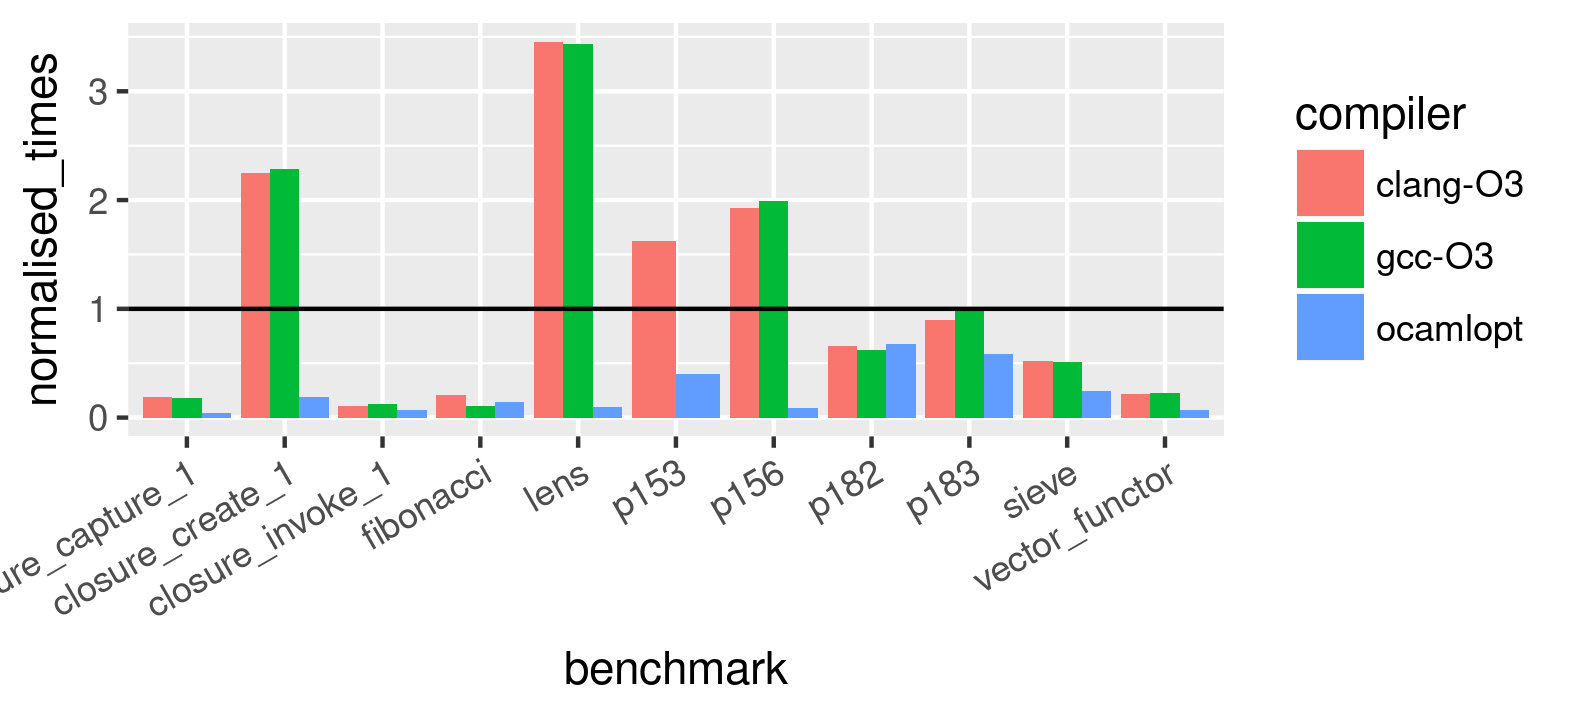
\includegraphics[width=16cm]{resultsummary-b477d4580}

\caption{Summary graph of performance for optimised configurations, relative to
the baseline ``ocaml'' bytecode compiler. The horizontal line at 1.0 normalised
time represents this baseline.}\label{graph-summary}
\end{figure}

\subsection{Microbenchmarks}
These microbenchmarks written from scratch by me. These test particular aspects
of the performance of the generated code.

\begin{enumerate}
  \item
    The \textbf{\texttt{closure\char`_create\char`_<n>}} family of benchmarks test the performance of
    creating closures which take $n$ arguments and capture 1 environment value.

    There are three interesting things to note from the results, graphed in figure \ref{graph-closure-create}:
    \begin{enumerate}
      \item performance is fairly constant for all values of $n$, for all compilers;
      \item however, creating closures is more than twice as slow for C
        compiled programs compared to the bytecode compiler. This is likely
        due to the overhead incurred in writing the 23/27 byte machine code stub
        for each closure;

      \item there is a small speed penalty when $n>5$. This
        corresponds to the case where extra machine code needs to be emitted to
        perform stack operations.

        It turns out that there is a long-standing
        bug in gcc which causes it not to merge sequential byte-sized store
        operations into a single wider store. This was verified by observing
        the generated assembly using Godbolt's compiler explorer
        \cite{godbolt}. The clang compiler does not suffer from this same
        issue.
    \end{enumerate}

    \begin{figure}[h]
\centering
  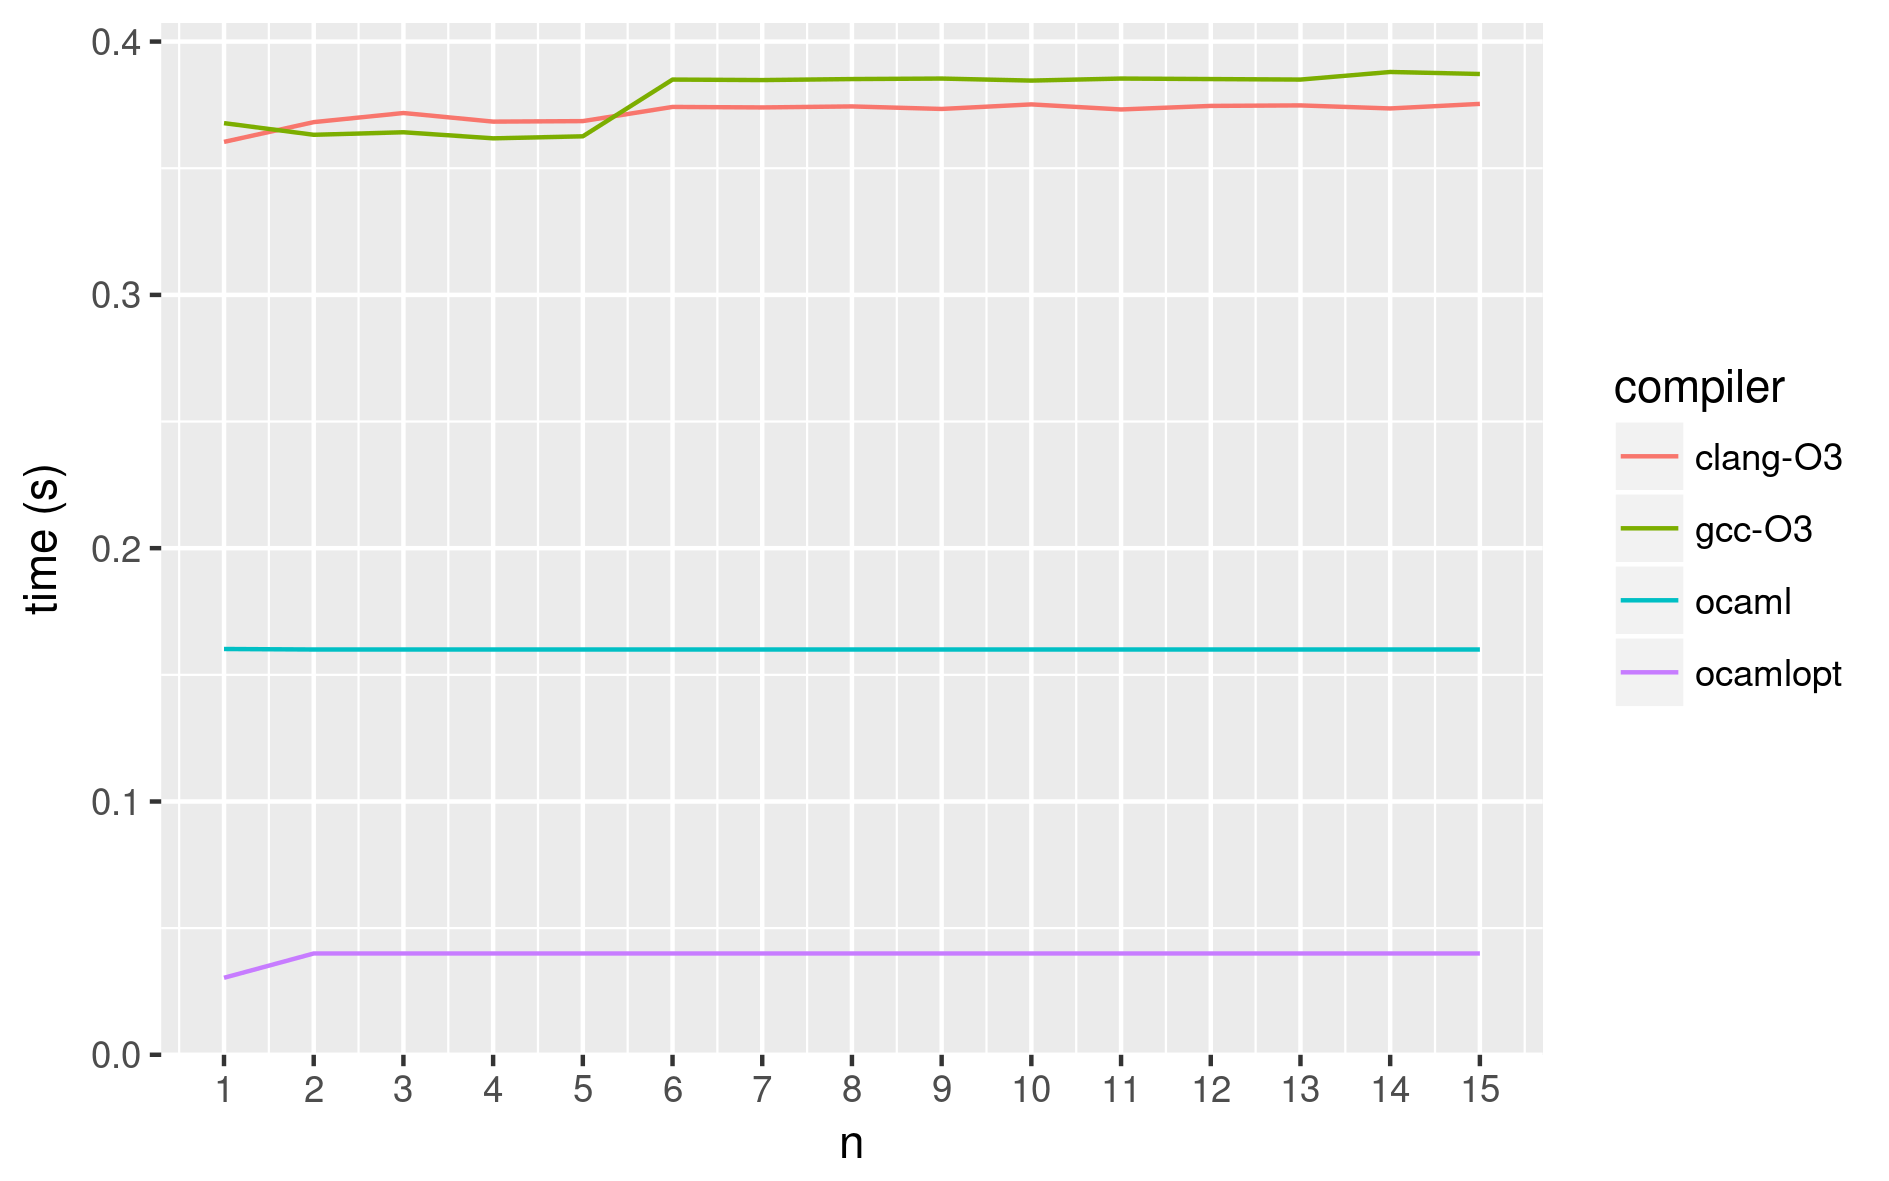
\includegraphics[width=16cm]{resultclosure_create_summary_all-b477d4580}

  \caption{\lstinline!closure_create_<n>! results.}\label{graph-closure-create}
\end{figure}


  \item
    The \textbf{\texttt{closure\char`_invoke\char`_<n>}} family of benchmarks the performance of
    invoking closures which take $n$ arguments and capture 1 environment value.

    The results are graphed in figures \ref{graph-closure-invoke} and
    \ref{graph-closure-invoke-opts}. From the first graph one can see that the
    OCaml bytecode is extremely slow (by a factor of more than 9 compared to
    the C compiled code) at invoking closures. It's more useful to look at the
    second graph, which only plots the optimised native code compiler configurations.

    The gcc results seem to be very noisy. However, it turns out that the
    standard error for each particular value of $n$ is extremely low,
    indicating that this ``noise'' seems to be deterministic and
    reproduceable. These are likely caused by cache-related effects.

    It's easier to draw conclusions from the clang results. When $n \le 5$,
    everything is passed in registers. This is effectively constant time, as expected.
    Invoking closures which take $n > 5$ arguments requires the compiler to place $n - 6$
    arguments on the stack.

    Interestingly, \lstinline!ocamlopt! seems to be able to execute the closure
    in constant time regardless of $n$. I suspect this is because the
    compiler backend has managed to optimise out the call through inlining.
    The gcc and clang compilers cannot see through the closure operation, so
    unfortunately they cannot perform same inlining operation.

    \begin{figure}[h]
\centering
  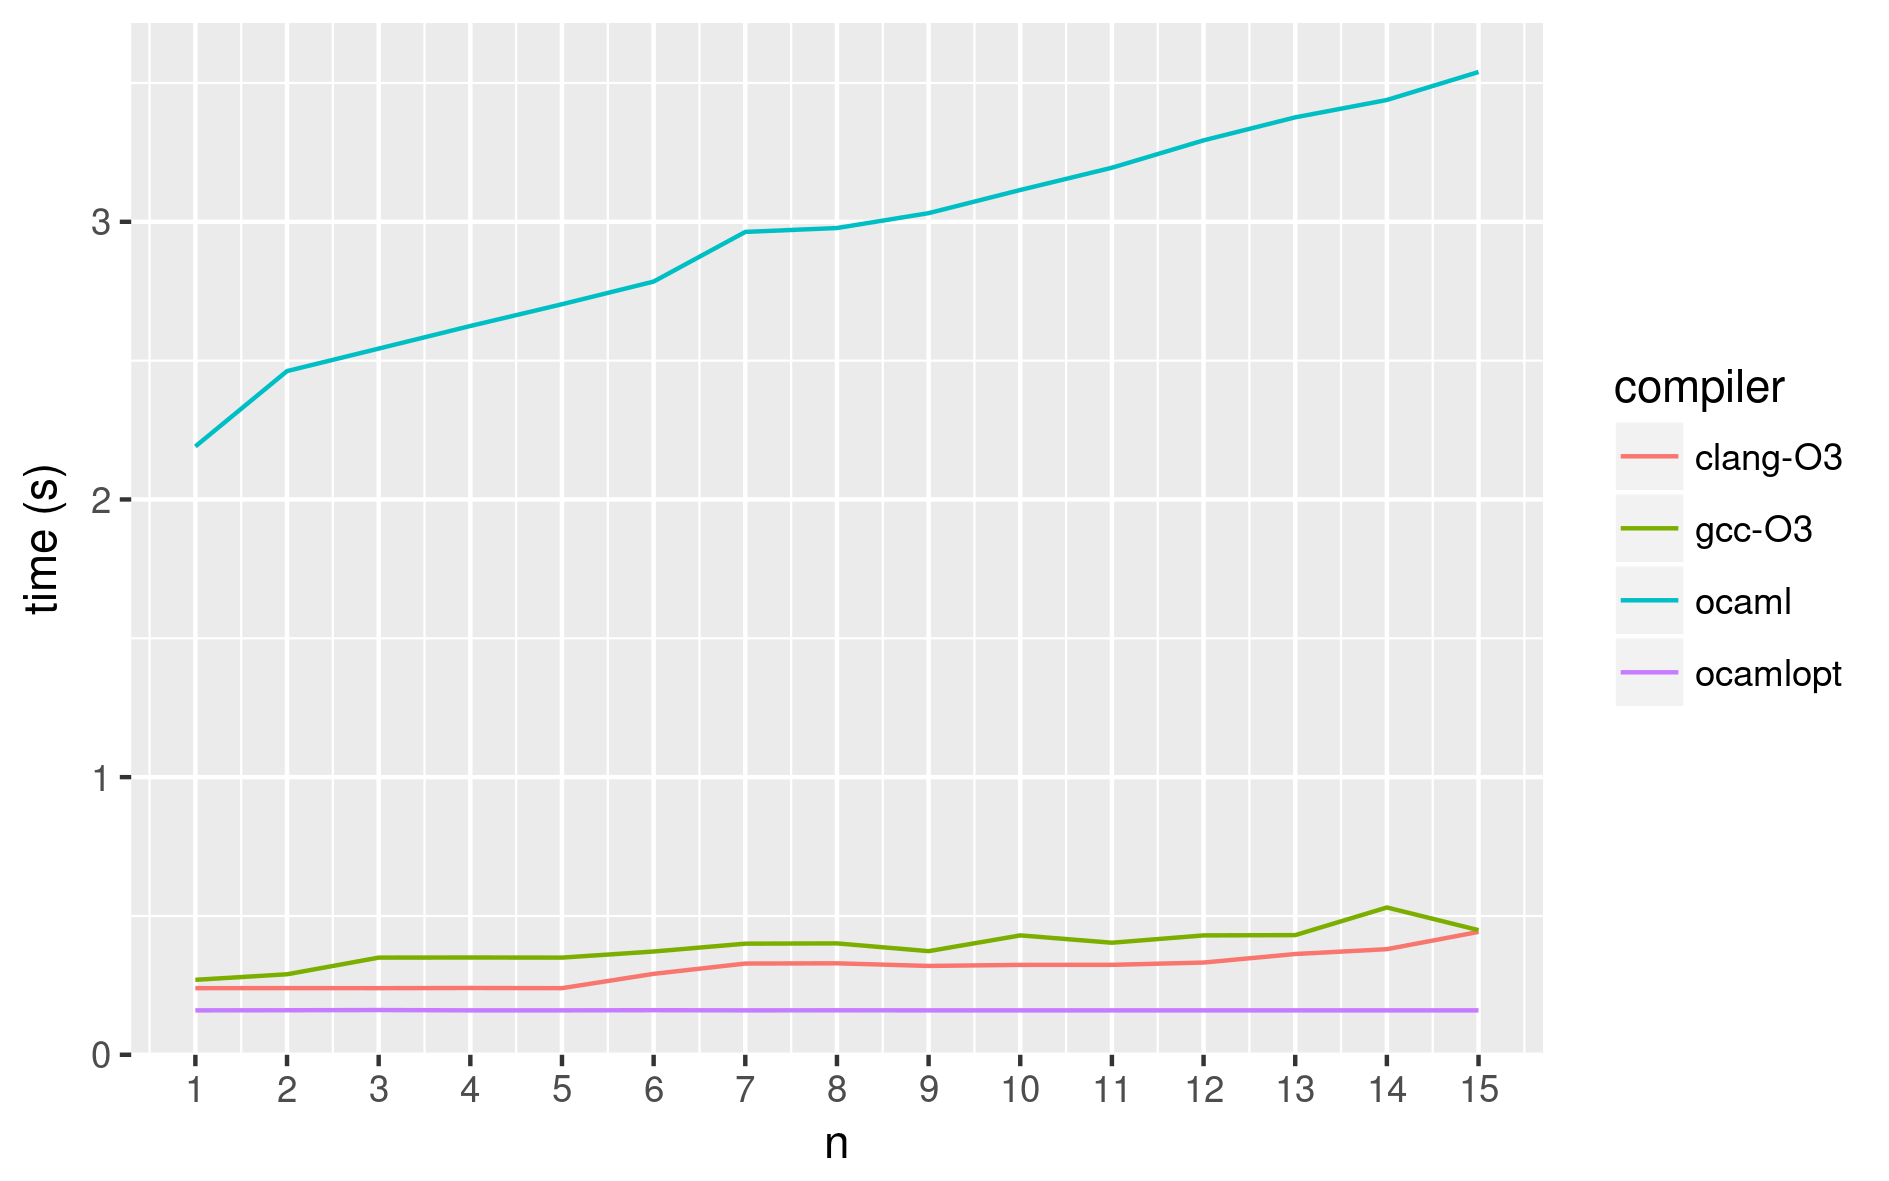
\includegraphics[width=16cm]{resultclosure_invoke_summary_all-b477d4580}

  \caption{\lstinline!closure_invoke_<n>! results.}\label{graph-closure-invoke}
\end{figure}

\begin{figure}[h]
\centering
  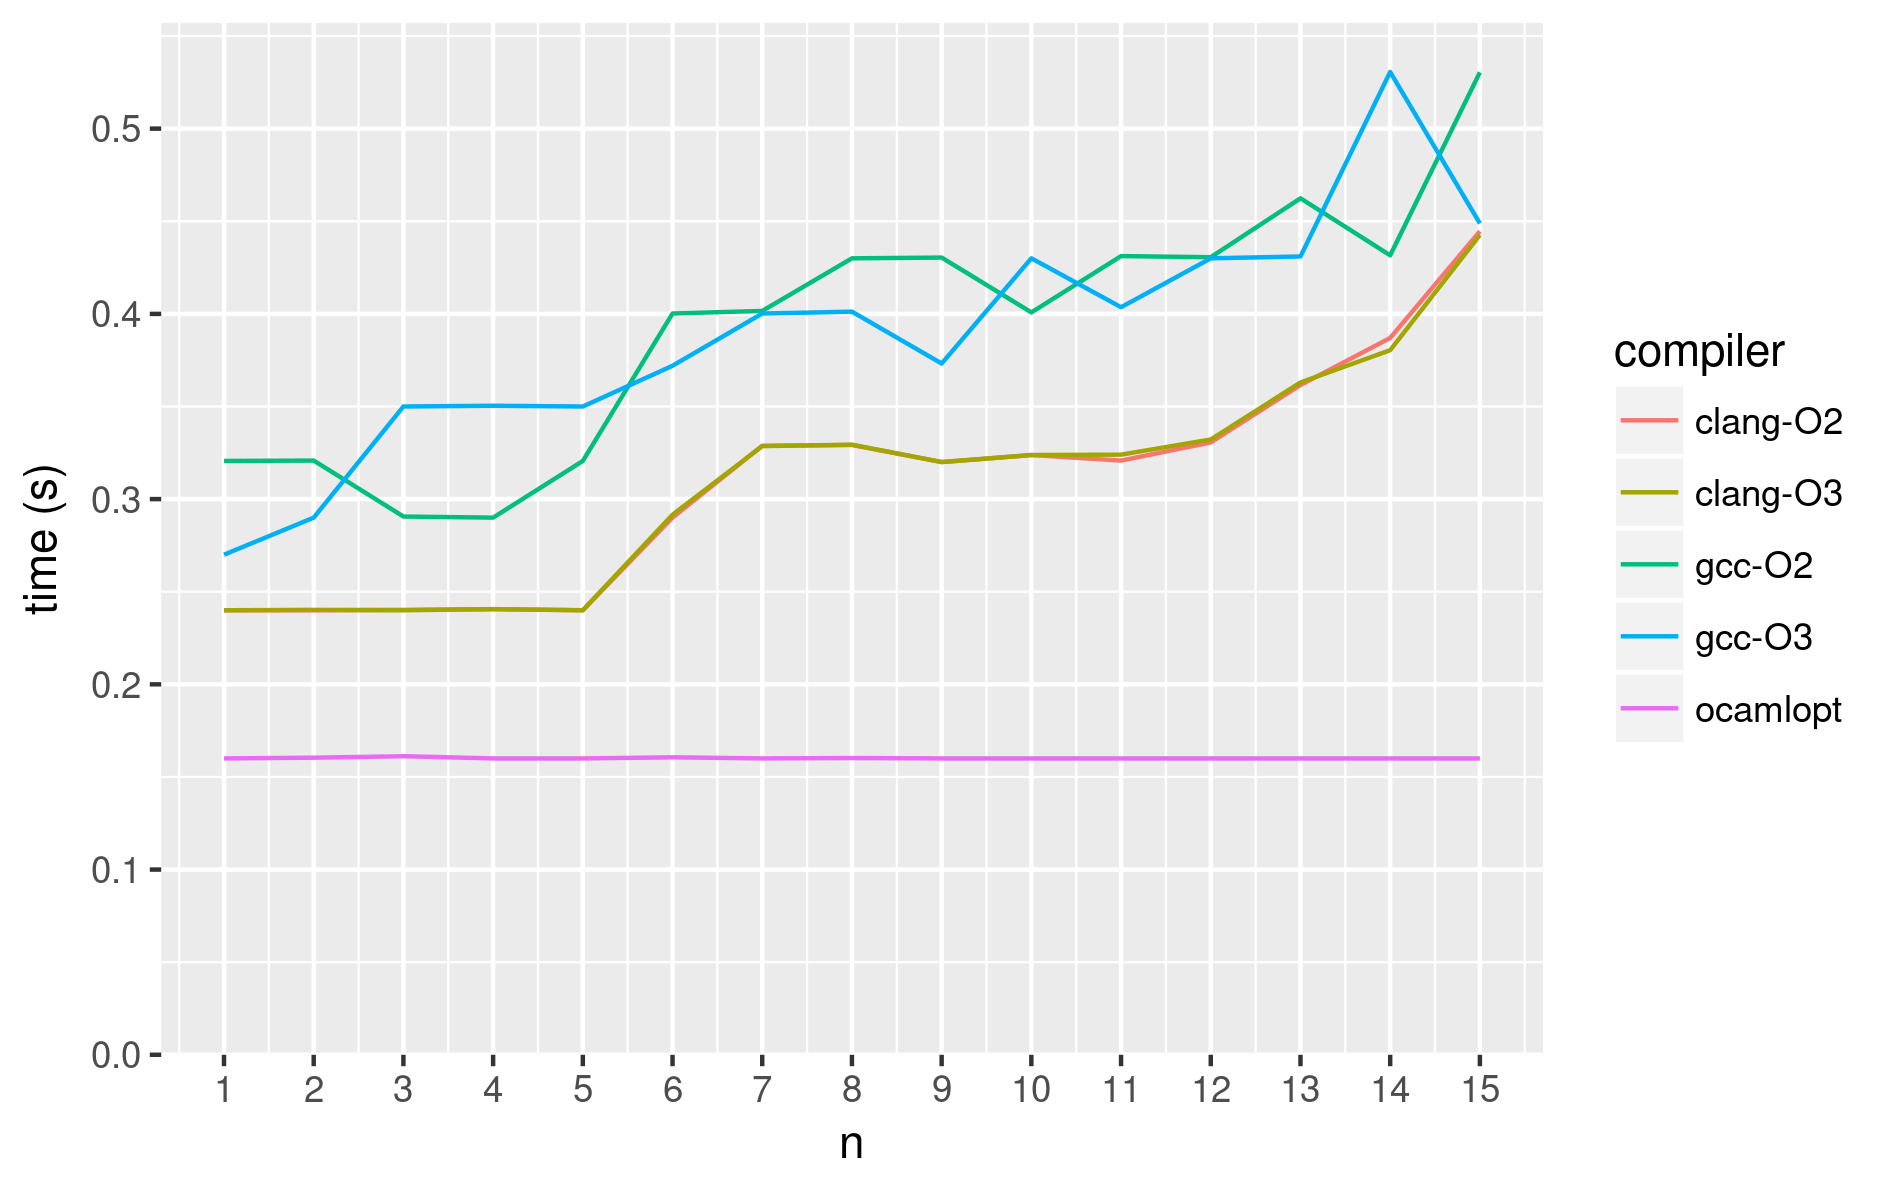
\includegraphics[width=16cm]{resultclosure_invoke_summary_opts-b477d4580}

  \caption{\lstinline!closure_invoke_<n>! results (optimised compilers only).}\label{graph-closure-invoke-opts}
\end{figure}


  \item
    The \textbf{\texttt{closure\char`_capture\char`_<n>}} family of benchmarks the performance
    of invoking closures which take 1 argument and capture $n$ variables from their environment.

    As my C compiler generates code which simply copies each captured variable
    into the environment object, I would expect time to increase linearly with $n$.
    This is indeed observed for each compiler configuration, although
    interestingly gcc seems to have a slope which is shallower than all others
    for the range of $n$ tested.

    \begin{figure}[h]
\centering
  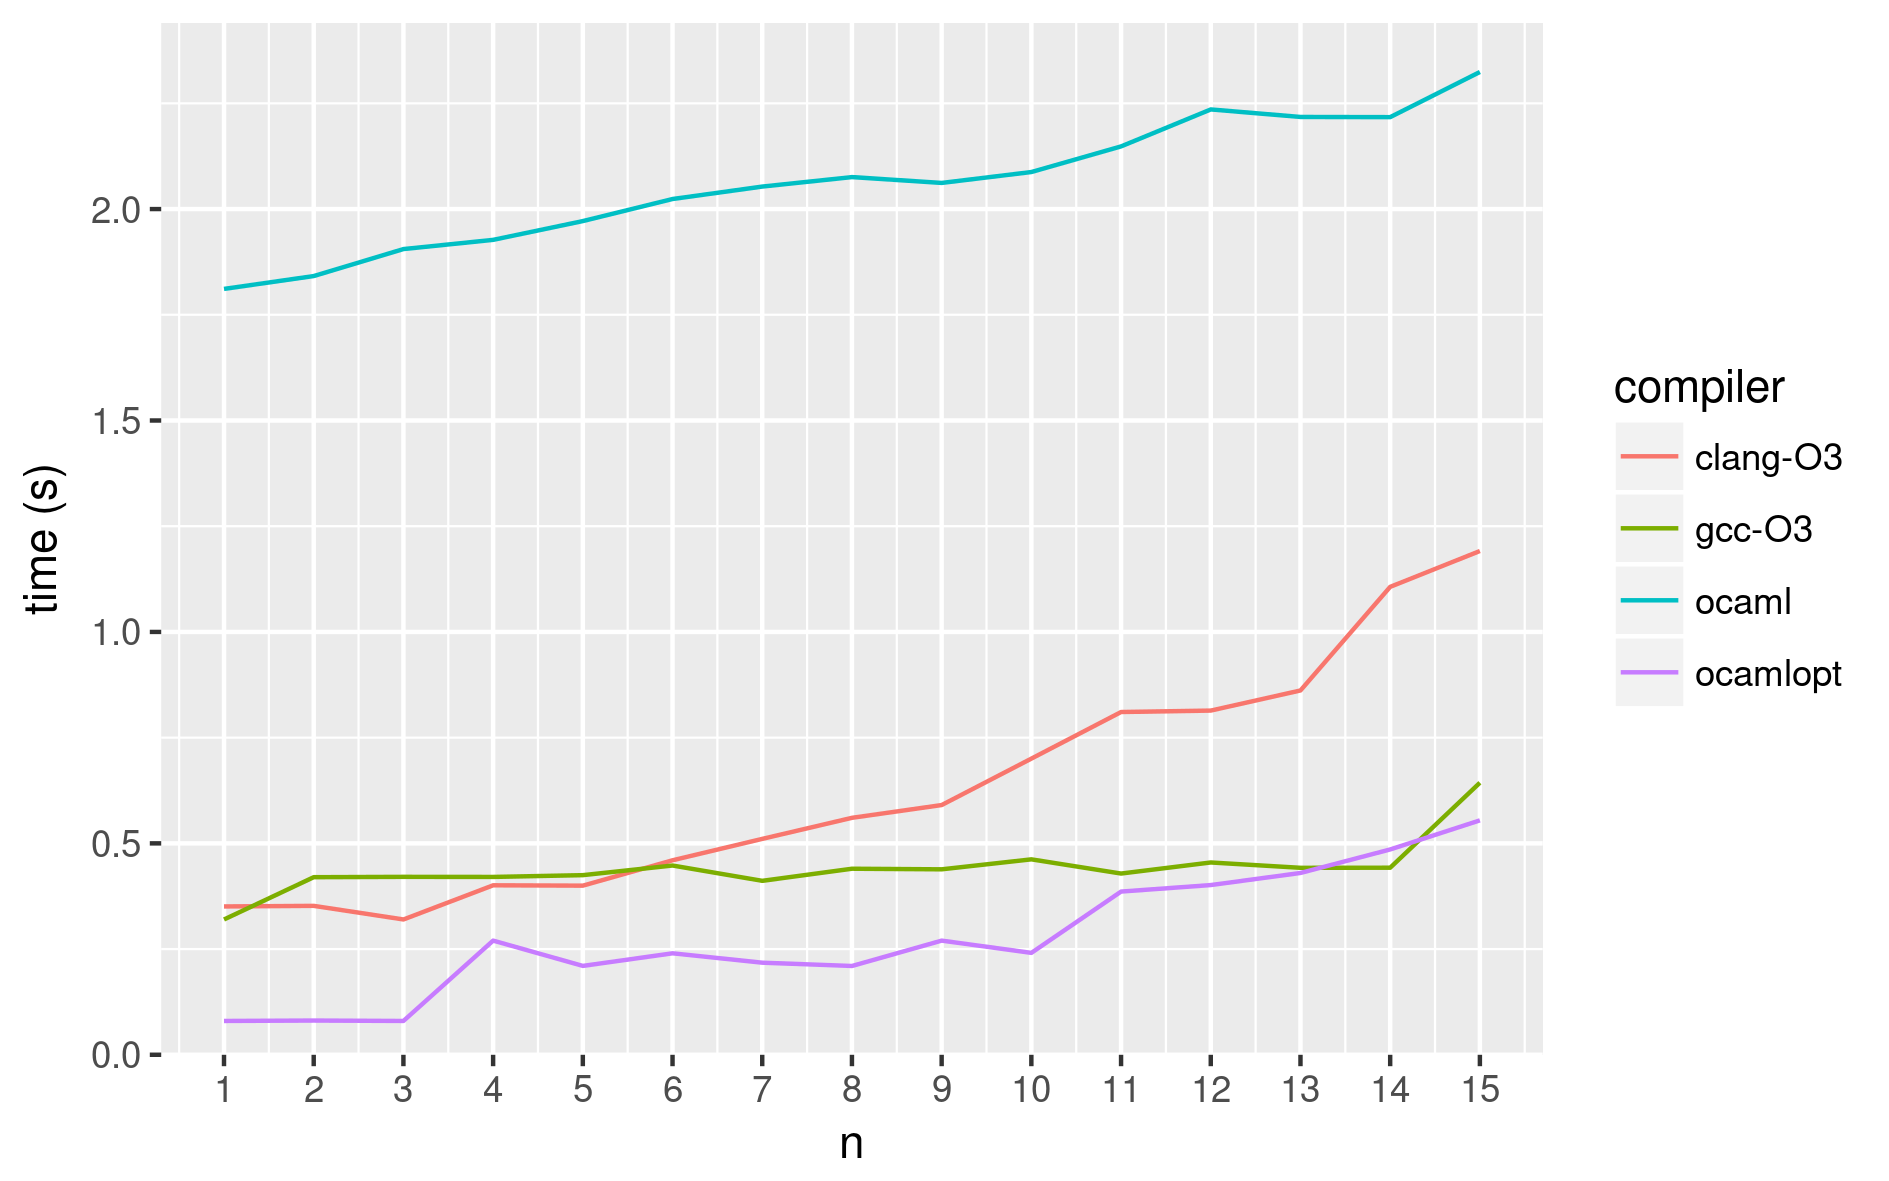
\includegraphics[width=16cm]{resultclosure_capture_summary_all-b477d4580}

  \caption{\lstinline!closure_capture_<n>! results.}\label{graph-closure-capture}
\end{figure}

  \item

  The \textbf{\texttt{list\char`_sort}} benchmark was written from scratch, to test the
  performance of the unmodified pure-OCaml standard library \lstinline!List.sort!
  routine (see section \ref{module-list}).

  The routine only creates a constant number of closures, but makes heavy use of
  closure invocation and allocates heavily.
\end{enumerate}

\subsection{\texttt{operf-micro} benchmark suite}
These are various sized benchmarks adapted from the OCamlPro's
      \lstinline!operf-micro! benchmark suite. These needed adapting before
      they could be used, due to being dependent on an OCaml-side framework
      which performs timing and measures GC statistics, features which are not
      supported by my compiler.
\begin{enumerate}

  \item
    The \textbf{\texttt{fibonacci}} benchmark was adapted from the \lstinline!fibonnaci!
[\textit{sic}] benchmark in \lstinline!operf-micro!.

This simple microbenchmark implements the naive (non-memoising) recursive
Fibonacci function, and uses it to evaluate the $40$-th Fibonacci number.

The benchmark primarily stress-tests the speed of function calls, as the cost
of invoking recursive calls dominates the amount of work done inside each call.

C compilers do an extremely good job with gcc beating out even the native OCaml compiler.

\item

  The \textbf{\texttt{lens}} benchmark implements a Haskell-style lens (otherwise known as
functional references), and then uses lenses to operate on a
\lstinline!rectangle! record type.

This makes usage of records and higher order functions, creating a very large
number of closures.

C compilers do unusually poorly on this benchmark; this motivated the
investigation in section \ref{performance-discrepancies}.

\item

  The \textbf{\texttt{sieve}} benchmark implements a linked-list sieve of Eratosthenes.

This benchmark performs many list operations and is very allocation-heavy.

\item

  The \textbf{\texttt{vector\char`_functor}} benchmark implements 2D and 3D vectors in two
different styles -- directly and by using a generic functor. It then uses these
implementations to create and calculate the dot product of $10^6$ 2D and 3D
vectors.

This benchmark allocates many records, and performs floating point operations.
\end{enumerate}

\subsection{Macrobenchmarks}
These are larger benchmarks written by me, as solutions to Project Euler problems.

\begin{enumerate}
\item

The \textbf{\texttt{p153}} benchmark makes usage of exceptions to break out of a recursive loop early.

\item
  The \textbf{\texttt{p156}} benchmark makes heavy use of recursion, closures and imperative-style \lstinline!for! loops.

\item
  The \textbf{\texttt{p182}} benchmark makes use of a tail-recursive GCD implementation, reference updates and imperative-style \lstinline!for! loops.

\item
  The \textbf{\texttt{p183}} benchmark makes heavy use of both integer and floating point arithmetic (\lstinline!log!, \lstinline!exp!, floating point division).
\end{enumerate}


\subsection{Investigating performance discrepancies}\label{performance-discrepancies}

\subsubsection{}

  The \lstinline!list_sort! and \lstinline!p153! benchmarks fail with a
  segmentation fault when compiled with \lstinline!clang -O0! or
  \lstinline!gcc! at all optimisation levels. The cause of this is a stack
  overflow from a lack of tail-call optimisation.

  On further investigation, I found the root cause, illustrated by the following C function:
\lc\begin{lstlisting}
int f(int x) {
  int ret;
  if (g(x)) {
    ret = f(x + 1);
  } else {
    ret = 42;
  }
  return ret;
}\end{lstlisting}\lnone{}
  With a small amount of optimisation, \lstinline!f(x + 1)! can be moved into
  tail call position. It is somewhat surprising that GCC fails to recognise
  and take advantage of this.

  \subsubsection{Instrumentation}

In order to dig deeper into why certain benchmarks seem perform significantly
worse than others, I decided to create a branch of my compiler with an
instrumented runtime which reported the following runtime statistics. If it turned out that
relative program performance were correlated with that program a specific high
statistic, this would point at a part of the runtime where my C implementation were
weaker than OCaml's.
\begin{enumerate}
  \item \textbf{number of allocations performed}. This is achieved by hooking
    into the \lstinline!malloc! function, by adding
    the following to the \lstinline!liballocs_runtime.h! header file:
    \lc\begin{lstlisting}
extern int n_allocations;
#define malloc(x) (++n_allocations, malloc(x))\end{lstlisting}\lnone

    (The counter \lstinline!n_allocations! is instantiated
    in \lstinline!liballocs_runtime.c!.)
  \item \textbf{number of closures created}. This is achieved by hooking into
    the \lstinline!ocaml_liballocs_close!  function, incrementing a counter
    each time the function is called.
  \item \textbf{number of times a closure was invoked}. This is tricker to
    instrument because unlike the previous two, there is no common function
    which is called when a closure is invoked. The code that we
    must insert instrumentation into is the generated code stub itself.

    In \lstinline!ocaml_liballocs_close!, we prefix the following two instructions to
    each generated code stub:
    \begin{lstlisting}
mov r11, <n_closures_invoked>
add dword [r11], 1\end{lstlisting}
    where \lstinline!n_closures_invoked! is the address of the counter variable.
\end{enumerate}

The results are shown in table \ref{tab-instrumentation}.

I discovered a strong correlation between a benchmark's slowness and its rate
of closure creation (total number of
closures created divided by the absolute amount of time taken). This is
clearly seen in the scatter diagram in figure \ref{fig-closure-create-scatter}.

I can conclude from this that the closure creation process
(\lstinline!ocaml_liballocs_close!) is likely the weak link in my runtime, in
comparison to upstream OCaml. It would be interesting to see whether this could
be optimised, and what effect this could have on the benchmarks.

\begin{table}
  \tiny
  \centering
  \begin{tabular}{c | c c | c c | c c}

benchmark & allocations & allocations/s & closures created & closure created/s & closures invoked & closures invoked/s \\ \hline
\lstinline!closure_capture_1! & 3 & 8.55 & 1 & 2.85 & $1.00\times 10^8$ & $2.85\times 10^8$ \\
\lstinline!closure_create_1! & $1.00\times 10^7$ & $2.78\times 10^7$ & $1.00\times 10^7$ & $2.78\times 10^7$ & 0 & 0 \\
\lstinline!closure_invoke_1! & 5 & 20.8 & 1 & 4.17 & $1.00\times 10^8$ & $4.16\times 10^8$ \\
\lstinline!fibonacci! & 9 & 13.8 & 0 & 0 & 0 & 0 \\
\lstinline!lens! & $1.90\times 10^7$ & $1.40\times 10^7$ & $1.20\times 10^7$ & $8.82\times10^6$ & $4.00\times10^6$ & $2.94\times10^6$ \\
\lstinline!list_sort! & $2.09\times 10^7$ & $3.11\times10^7$ & 5 & 7.45 & $2.05\times 10^7$ & $3.06\times10^7$ \\
\lstinline!p153!           & $4.48\times10^6$ & $6.90\times10^6$ & $2.48\times10^6$ & $3.82\times10^6$ & $1.44\times10^7$ & $2.22\times10^7$ \\
\lstinline!p156!           & $1.85\times10^7$ & $9.36\times10^6$ & $8.41\times10^6$ & $4.25\times10^6$ & $3.80\times10^7$ & $1.92\times10^7$ \\
\lstinline!p182!           & $10$ & $13.7$ & $0$ & $0$ & $0$ & $0$ \\
\lstinline!p183!           & $3.00\times10^6$ & $7.50\times10^6$ & $1.00\times10^6$ & $2.50\times10^6$ & $2.00\times10^6$ & $5.00\times10^6$ \\
\lstinline!sieve!          & $3.91\times10^7$ & $2.72\times10^7$ & $4.90\times10^3$ & $3.40\times10^3$ & $3.86\times10^7$ & $2.68\times10^7$ \\
\lstinline!vector_functor! & $4.00\times10^7$ & $3.01\times10^7$ & $17$ & $12.8$ & $4.00\times10^7$ & $3.01\times10^7$
  \end{tabular}
  \caption{Instrumentation results. The per-second results are obtained by dividing the absolute values by the \lstinline!clang -O3! run time in seconds.}
  \label{tab-instrumentation}
\end{table}

\begin{figure}[h]
  \centering
  \includegraphics[width=15cm]{closure_create_scatter}
  \caption{A scatter plot of all benchmarks: plotting the normalised time against the rate of closure creation.}
  \label{fig-closure-create-scatter}
\end{figure}


\chapter{Conclusion}\label{conclusion}

The project was technically challenging, as I had to work with an unfamiliar
compiler's internals, as well as implementing a new backend from scratch.

My original motivations for this project were the following:
\begin{enumerate}
    \item \textbf{Feasibility}: my project was completely successful in
      demonstrating that compiling OCaml into C code is a feasible task. Many
      OCaml constructs are already supported, and the ones that are not
      (detailed below) were mostly omitted due to time constraints, rather than
      technical ones;
    \item \textbf{Performance}: despite not worrying specifically about
      generating performant C code in my compiler, the benchmarks show that
      the compiled C executables already perform competitively -- matching or
      exceeding OCaml bytecode performance in most cases, when closure creation
      doesn't dominate runtime;
    \item \textbf{Observability}: this was one of the weaker points of my
      project. Although observability through parametric polymorphism was
      achieved (section \ref{debugging}), I did not teach liballocs enough about OCaml
      types, which meant that values had to be printed as their raw in-memory representation.
      In hindsight I would have allocated more time working with
      \lstinline!Liballocs! to get the best results here, instead of focusing
      so much on making the compiler as complete as possible;
    \item \textbf{Portability}: my closure implementation in its current state
      hinders portability by assuming the generated code is being
      run on 64-bit Linux. Because of this
          I somewhat regret my choice of implementing closures from scratch --
          if I had taken advantage of a widely-ported library such as
          \lstinline!libffi!, then portability would have been completely
          achievable.
\end{enumerate}

There are still many limitations on my compiler that I'd
hypothetically like to fix:

\begin{itemize}
  \item Currently ``overapplication'' is unsupported. This is when the number of
      arguments provided to a function application exceeds the arity of the function being applied. This is illustrated by the
      following example:
      \lml\begin{lstlisting}
let f x = fun y -> 42
let overapplied = f 10 20\end{lstlisting}\lnone{}
      The C code this translates to would have to split this into two function
      calls, one after the other.

      The mechanism for detecting this situation is actually implemented in my
      compiler, however I did not have time to implement the actual translation.
  \item Block tags are not supported, which basically means that
      variant constructors which take arguments (e.g.
      \lstinline!Foo of int | Bar of string!) cannot currently be created. The
      issue is that my blocks do not have headers, so there is no space to
      store the tag byte. There are three possibilities I can think of to implement this, each with various tradeoffs:
      \begin{enumerate}
          \item add a header to all tags. This could cause a significant memory requirement increase;
          \item use a field in \lstinline!liballocs!'s \lstinline!uniqtype!
              structure, which is used to describe a particular allocation.
              This is space efficient because \lstinline!uniqtype!s are created
              per allocation-site rather than per runtime allocation. One
              downside is that \lstinline!liballocs! would become a hard
              dependency (which it currently isn't), which may hinder
              portability somewhat.
          \item use some spare bits in the NaN boxed value representation to
              store the tag. By squeezing out every single bit we possibly can,
              we can theoretically recover 6 bits for a tag (3 bits from the
              8-byte alignment requirement on pointers, 1 sign bit and 2
              mantissa bits from filling up the unused range as fully as
              possible). The advantage of this approach is that no extra memory
              is required at all. However the (significant) downside is that
              pointers must be masked before dereference, which likely incurs a
              significant performance penalty.
      \end{enumerate}
  \item Large parts of the standard library are unimplemented. Significantly
      \lstinline!Array! is missing, which provides a fixed-size contiguous list
      datatype.

      In fact, the \lstinline!array! datatype is builtin to the compiler, and there
      are many primitive \lstinline!Lambda! operations that operate on these.
      I did not have time to implement these. (This task is made even more tricky by
      the fact that there is a different layout of \lstinline!array! for doubles,
      and this optimisation is embedded deep into the compiler, bringing with it
      its own set of primitive operations and quirks.)
  \item Currently OCaml's polymorphic comparisons are unsupported, but all of the
      underlying techniques required to implement this are in place already. An
      implementation of this would use the \lstinline!IS_*! discriminating
      macros on NaN-boxed values to perform the correct comparison operation for
      the type of value stored.
\end{itemize}


%%%%%%%%%%%%%%%%%%%%%%%%%%%%%%%%%%%%%%%%%%%%%%%%%%%%%%%%%%%%%%%%%%%%%
% the bibliography
\begin{thebibliography}{1}

\bibitem{tarditi90}
  D. Tarditi, A. Acharya, P. Lee,
  \emph{No Assembly Required: Compiling Standard ML to C},
  November 1990. \\ \url{http://repository.cmu.edu/cgi/viewcontent.cgi?article=3011&context=compsci}

\bibitem{kell}
  Stephen Kell,
  \emph{liballocs},
  \\ \url{https://github.com/stephenrkell/liballocs}

\bibitem{breuel88}
  Thomas Breuel,
  \emph{Lexical Closures for C++},
  In Proc. USENIX C++ Conf., pages 293-304,
  Denver, CO, October 1988.  \\ \url{http://www.cl.cam.ac.uk/~srk31/teaching/redist/breuel88lexical.pdf}

\bibitem{jscore}
  WebKit authors,
  \emph{JSValue.h}.
  \\ \url{https://github.com/WebKit/webkit/blob/master/Source/JavaScriptCore/runtime/JSCJSValue.h}

\bibitem{godbolt}
  Matt Godbolt,
  \emph{Godbolt compiler explorer}.
  \\ \url{https://godbolt.org/}

\bibitem{dolan16}
  Stephen Dolan,
  \emph{Malfunctional Programming},
  ML Workshop, 2016.  \\ \url{https://www.cl.cam.ac.uk/~sd601/papers/malfunction.pdf}

\end{thebibliography}

%%%%%%%%%%%%%%%%%%%%%%%%%%%%%%%%%%%%%%%%%%%%%%%%%%%%%%%%%%%%%%%%%%%%%
% the appendices
\appendix

%\chapter{Latex source}
%
%\section{diss.tex}
%{\scriptsize\verbatiminput{diss.tex}}
%
%\section{proposal.tex}
%{\scriptsize\verbatiminput{proposal.tex}}
%
%\chapter{Makefile}
%
%\section{makefile}\label{makefile}
%%{\scriptsize\verbatiminput{makefile.txt}}
%
%%\section{refs.bib}
%%{\scriptsize\verbatiminput{refs.bib}}
%
%
\chapter{Project Proposal}

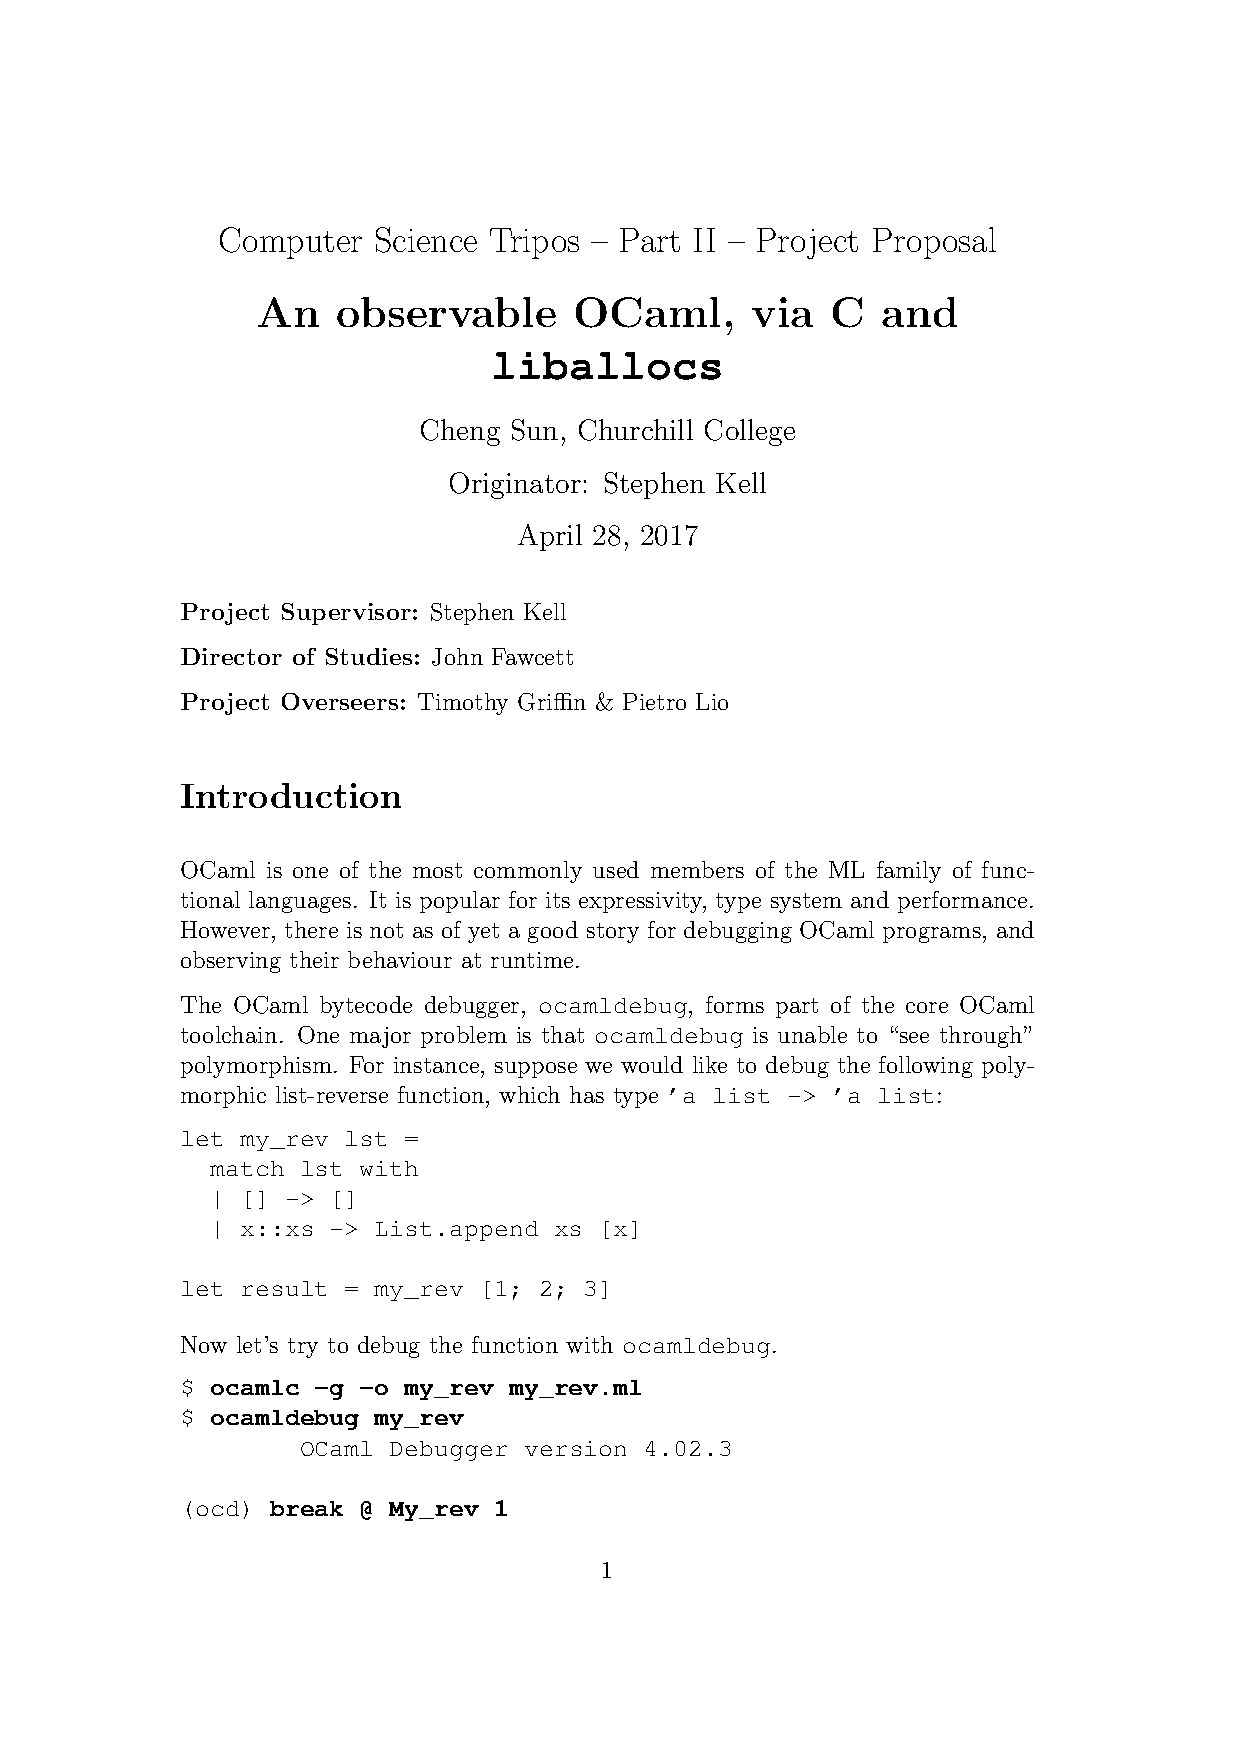
\includepdf[pages=-]{proposal.pdf}

\end{document}
